\chapter*{L’Equateur, de Baños à Quito\markboth{L’Equateur, de Baños à Quito}{}}
\section*{29 juin 2015}
Je quitte Baños par la route des cascades qui descend vers l'Amazonie sur 60km. 

\begin{center} 
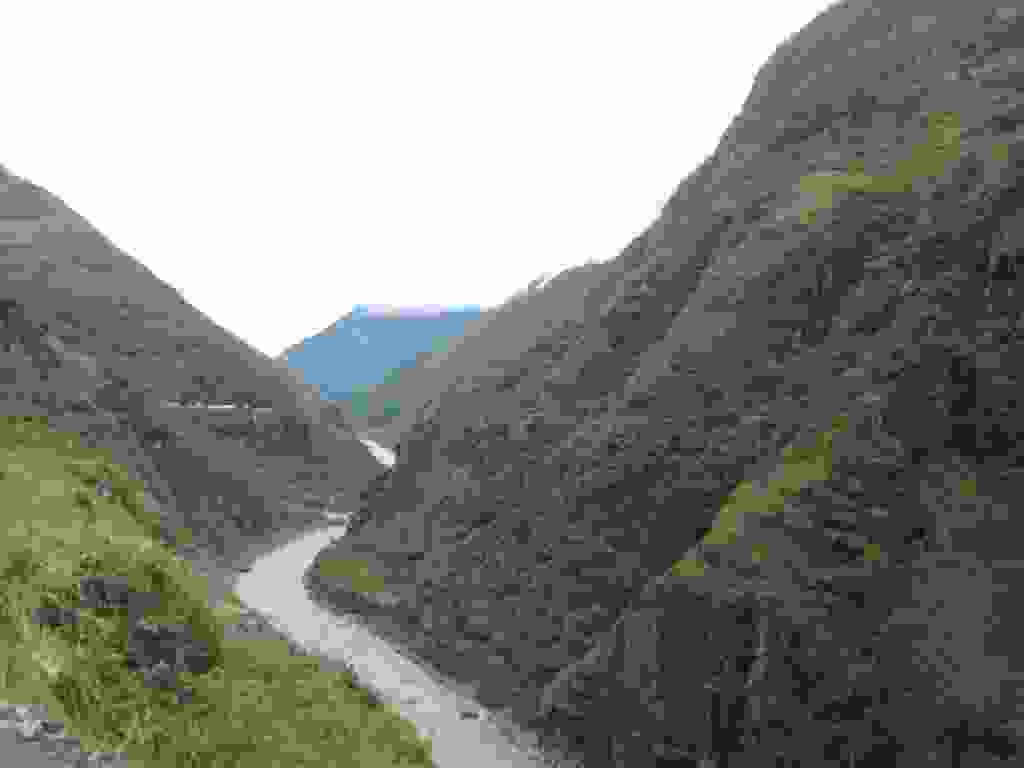
\includegraphics[width=\mywidth]{../wp-content/uploads/2015/06/wpid-wp-1435593846148-1024x768.jpg} 
\end{center}
\begin{center} 
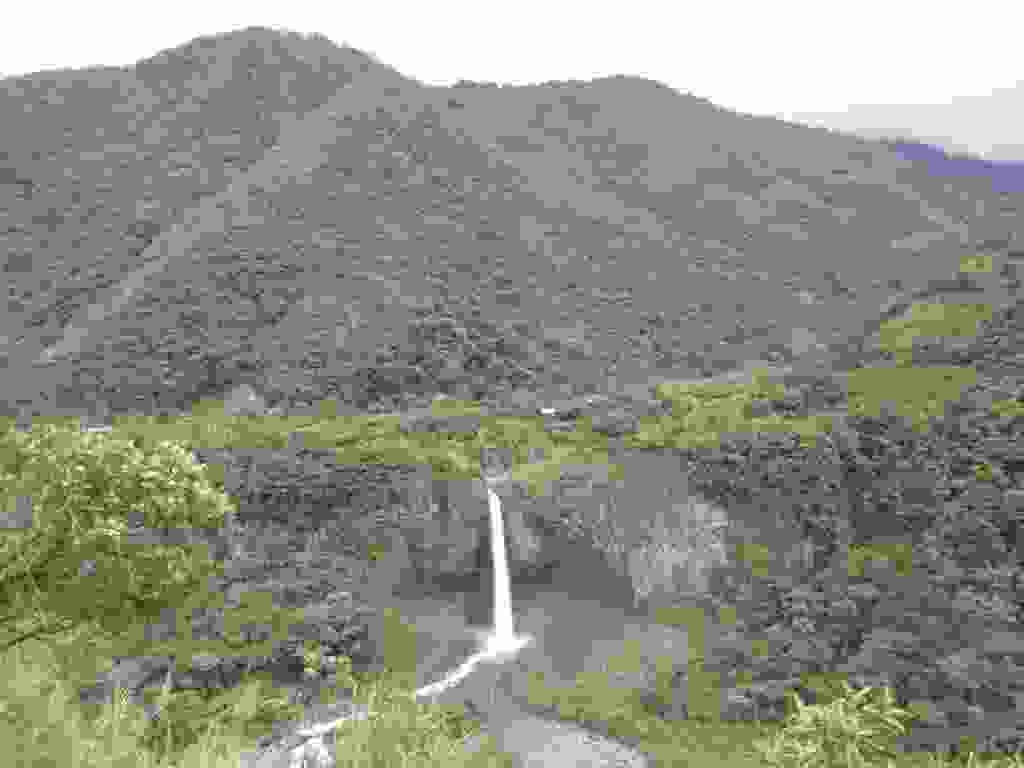
\includegraphics[width=\mywidth]{../wp-content/uploads/2015/06/wpid-wp-1435593861799-1024x768.jpg} \end{center}

La cascade Pailon del Diablo est la plus impressionnante. 
\begin{center} 
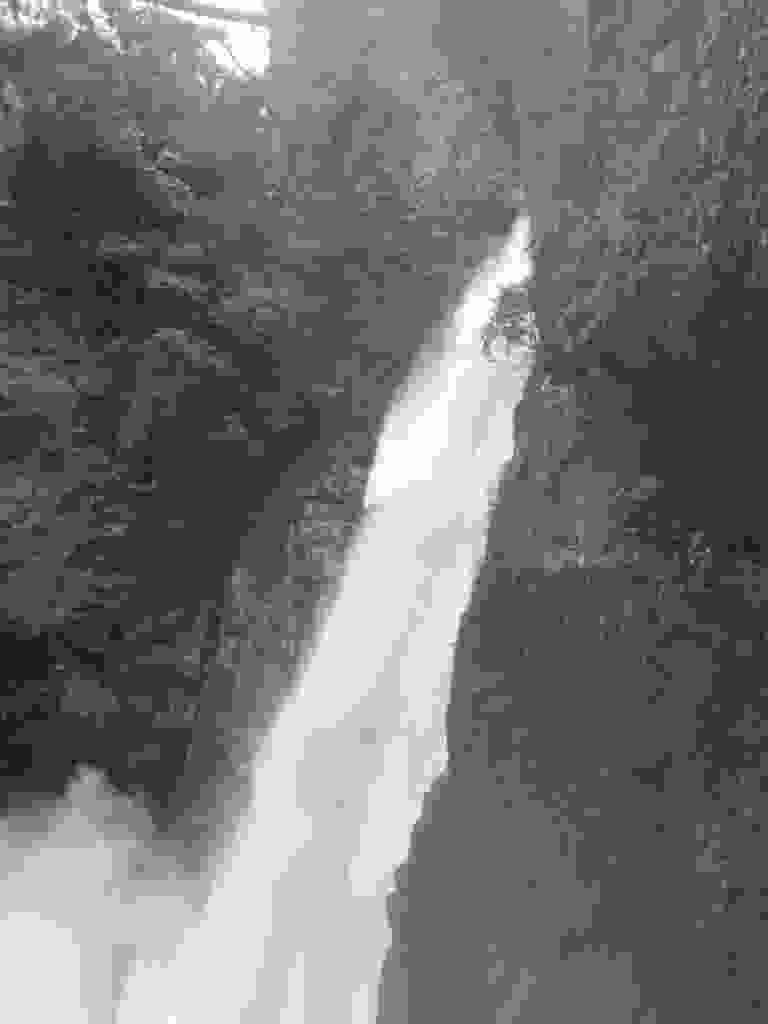
\includegraphics[height=\mywidth]{../wp-content/uploads/2015/06/P6224978-e1435962282463-768x1024.jpg} 
\end{center}
\begin{center} 
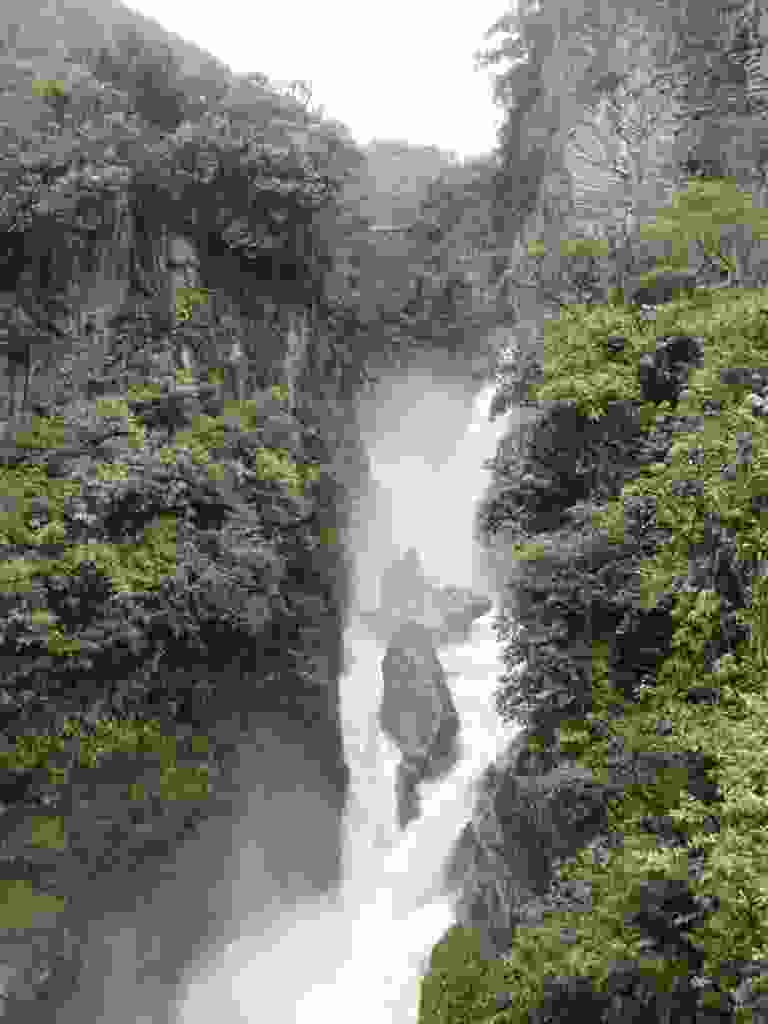
\includegraphics[height=\mywidth]{../wp-content/uploads/2015/06/P6224991-e1435962256922-768x1024.jpg} 
\end{center}

J'arrive à Puyo, une petite ville située à l'entrée de la jungle. 
\begin{center} 
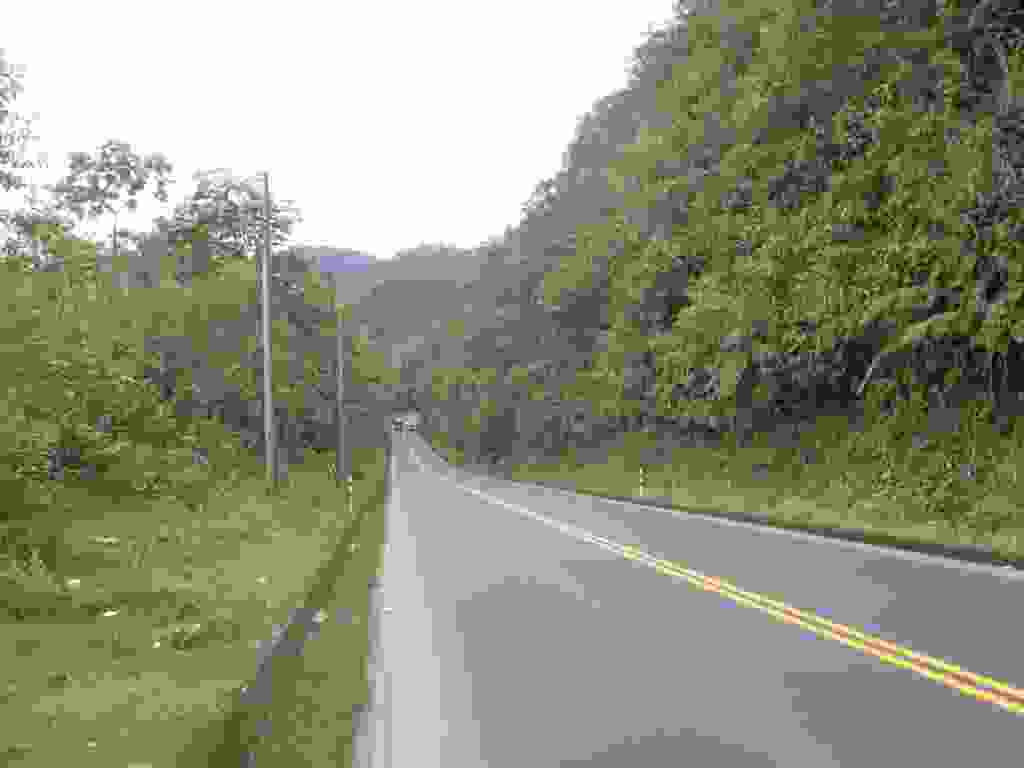
\includegraphics[width=\mywidth]{../wp-content/uploads/2015/06/P6224994-1024x768.jpg} 
\end{center}
\begin{center} 
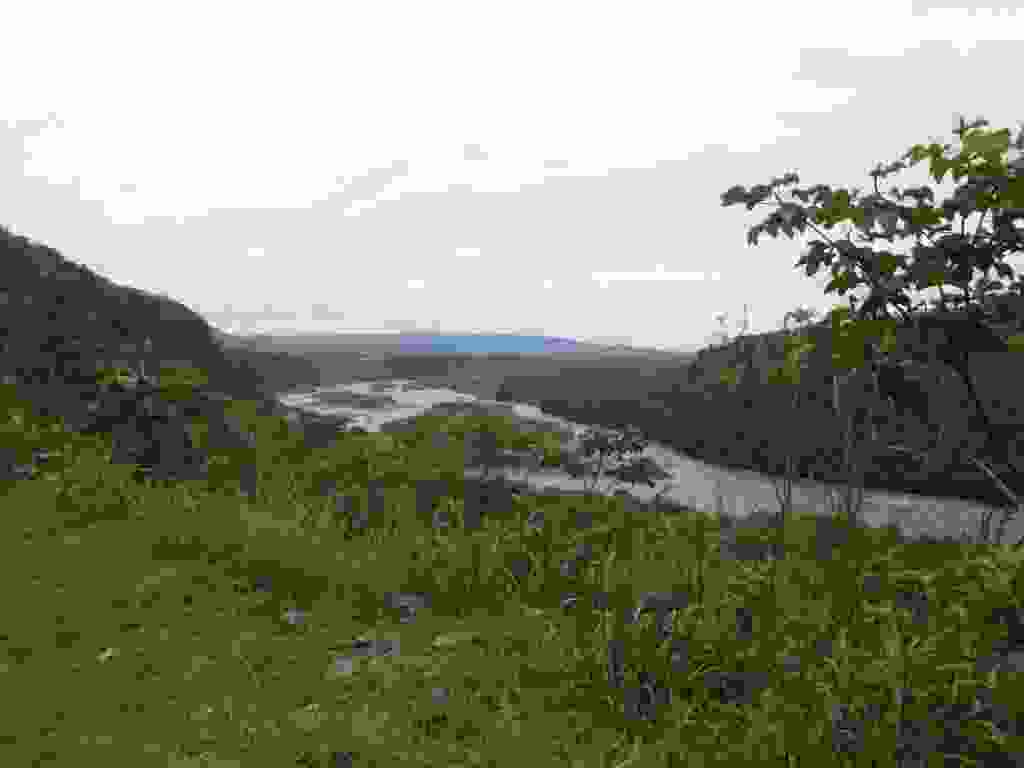
\includegraphics[width=\mywidth]{../wp-content/uploads/2015/06/P6224995-1024x768.jpg} 
\end{center}

J'en profite pour passer une journée dans la jungle avec un guide local, Enrique. La marche passe par deux belles cascades et on peut se baigner dans la seconde. 
\begin{center} 
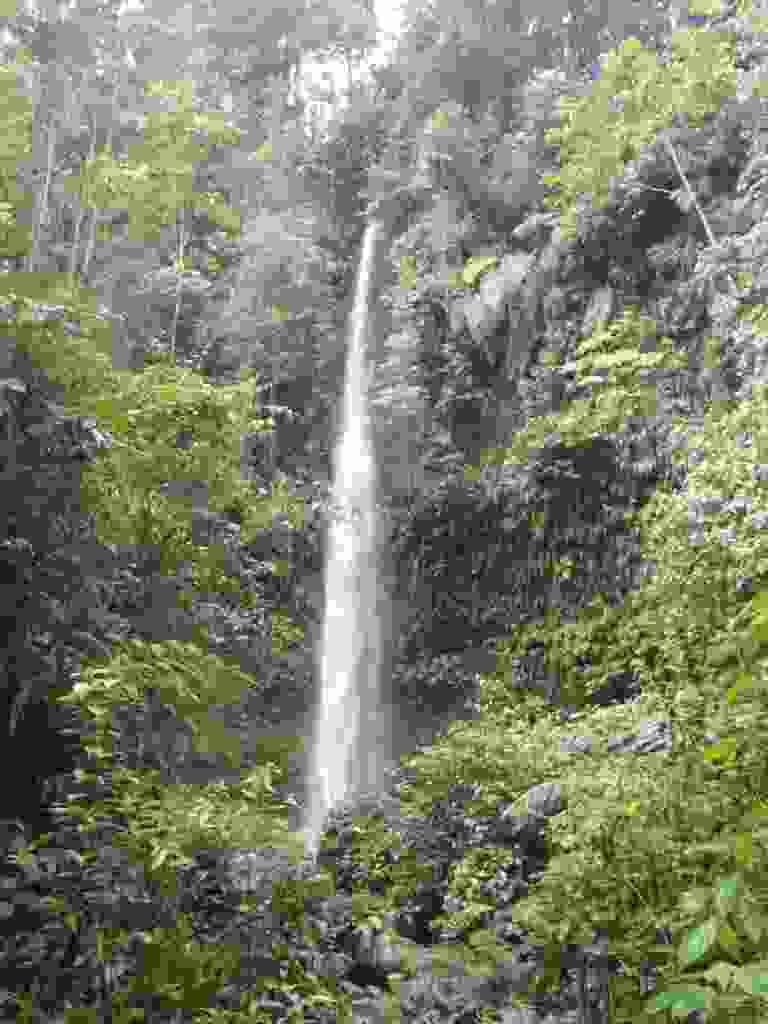
\includegraphics[width=0.6\textwidth]{../wp-content/uploads/2015/06/P6235001-768x1024.jpg} \end{center}
\begin{center} 
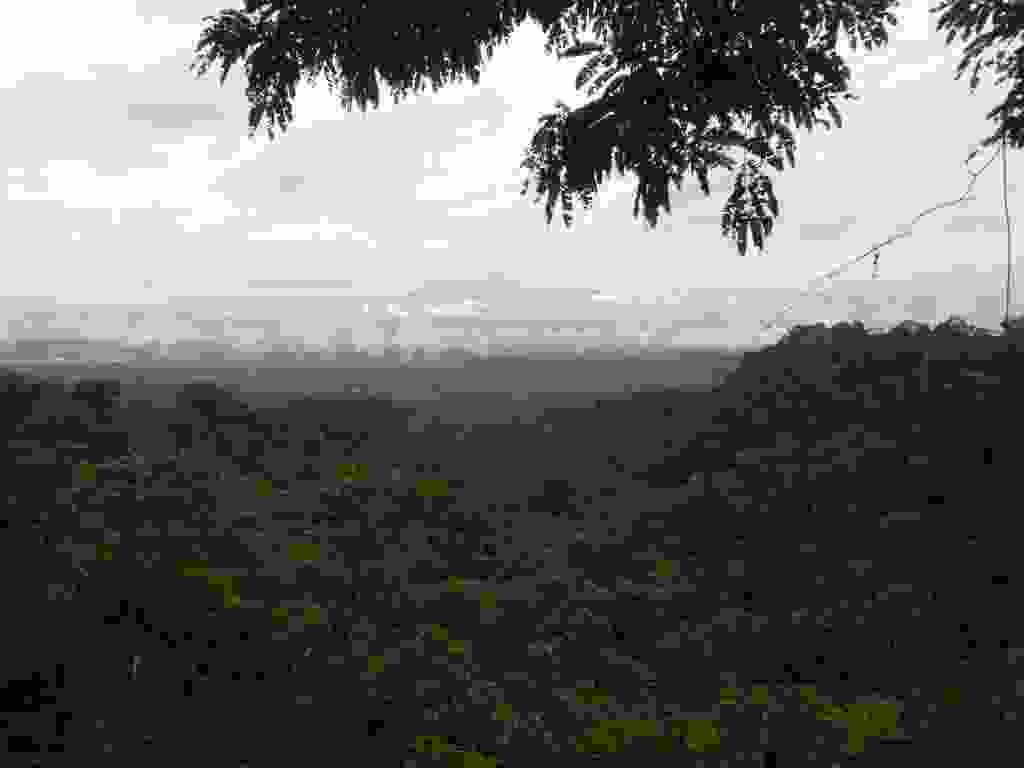
\includegraphics[width=\mywidth]{../wp-content/uploads/2015/06/P6235014-1024x768.jpg} 
\end{center} 
\begin{center} 
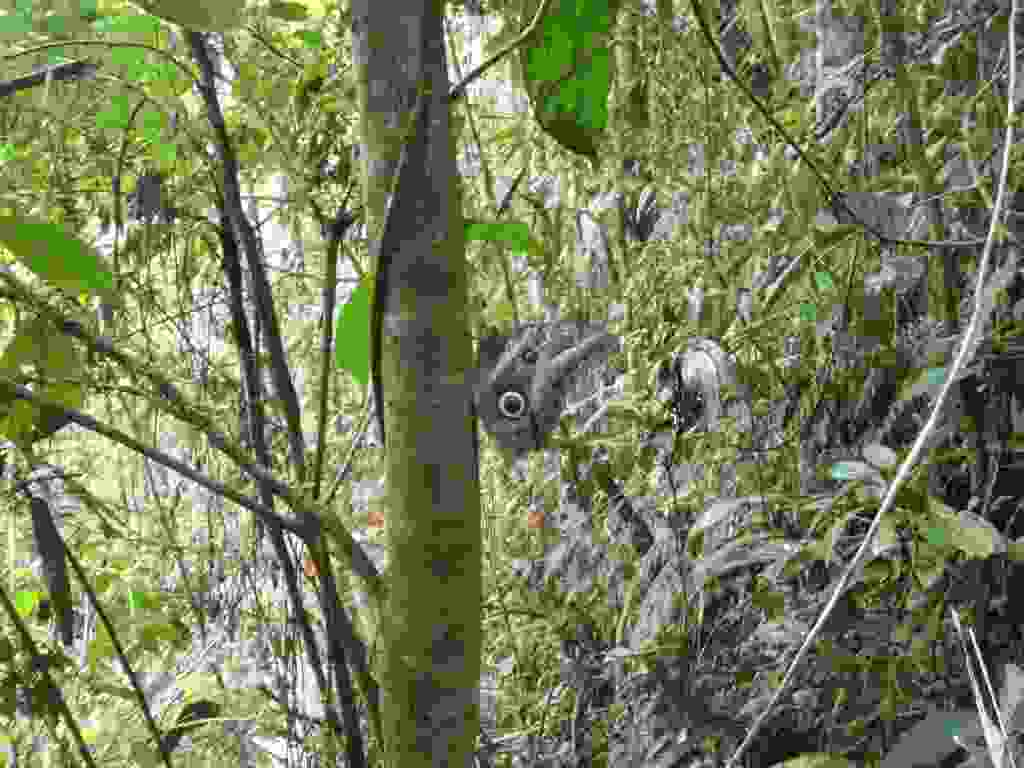
\includegraphics[width=\mywidth]{../wp-content/uploads/2015/06/P6235015-1024x768.jpg} 
\end{center}
\begin{center} 
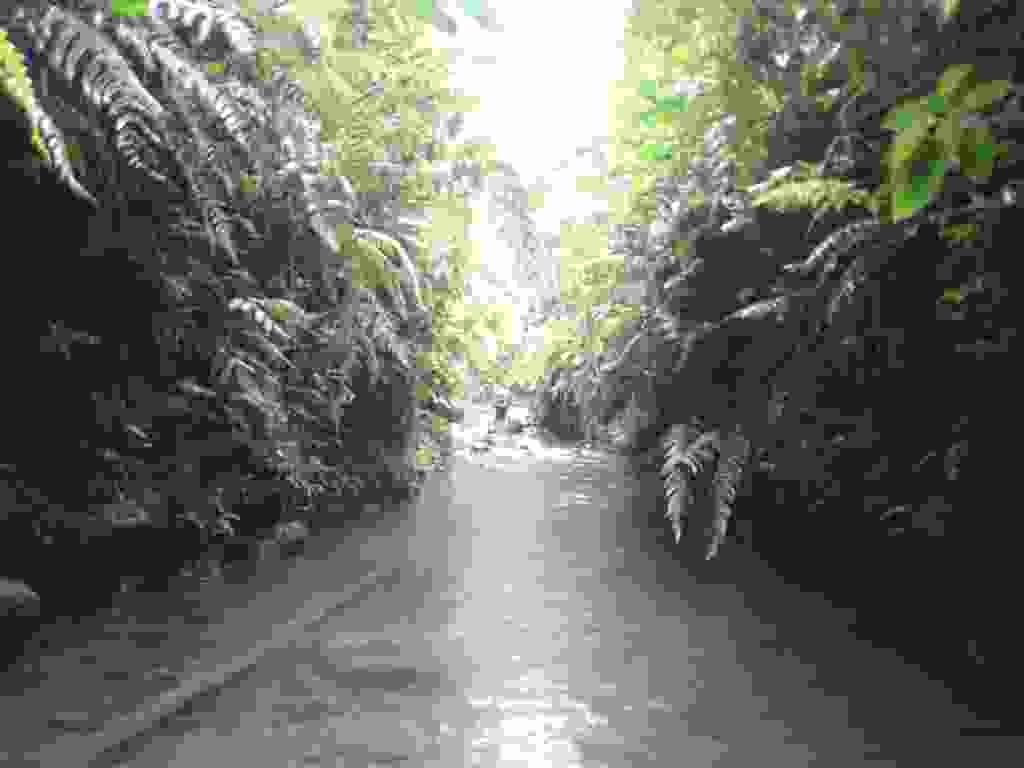
\includegraphics[width=\mywidth]{../wp-content/uploads/2015/06/P6235017-1024x768.jpg} 
\end{center}
\begin{center} 
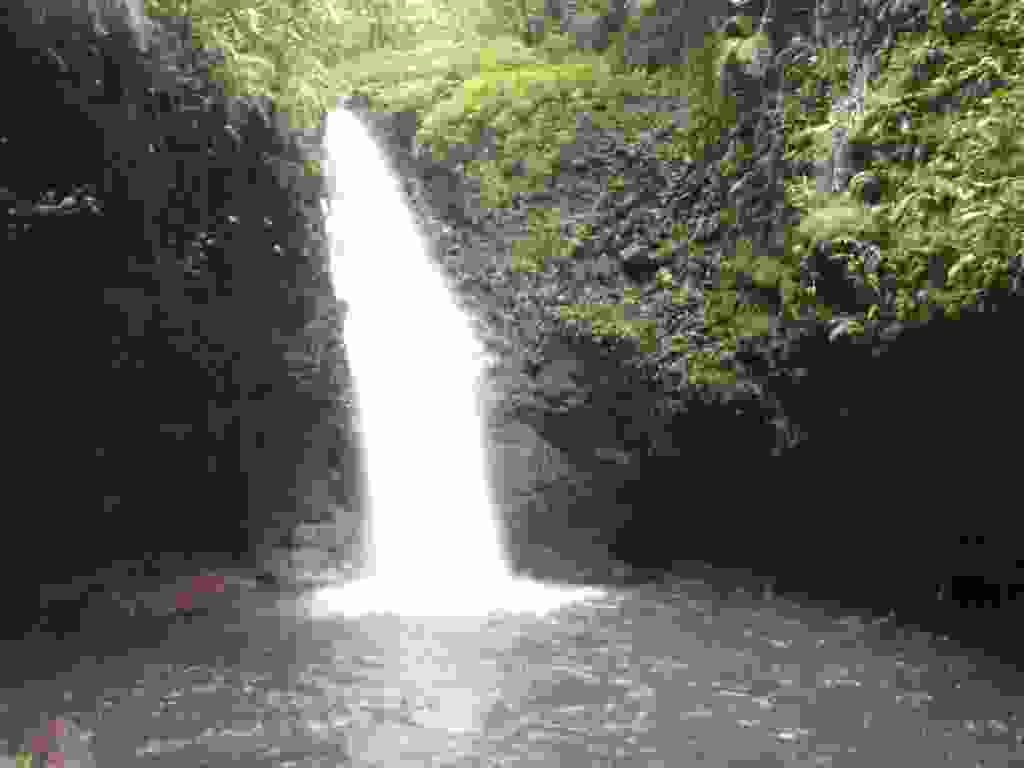
\includegraphics[width=\mywidth]{../wp-content/uploads/2015/06/P6235020-1024x768.jpg} 
\end{center}
\pagebreak

Des dizaines d'oiseaux qui s'envolent quand on arrive. 
\begin{center} 
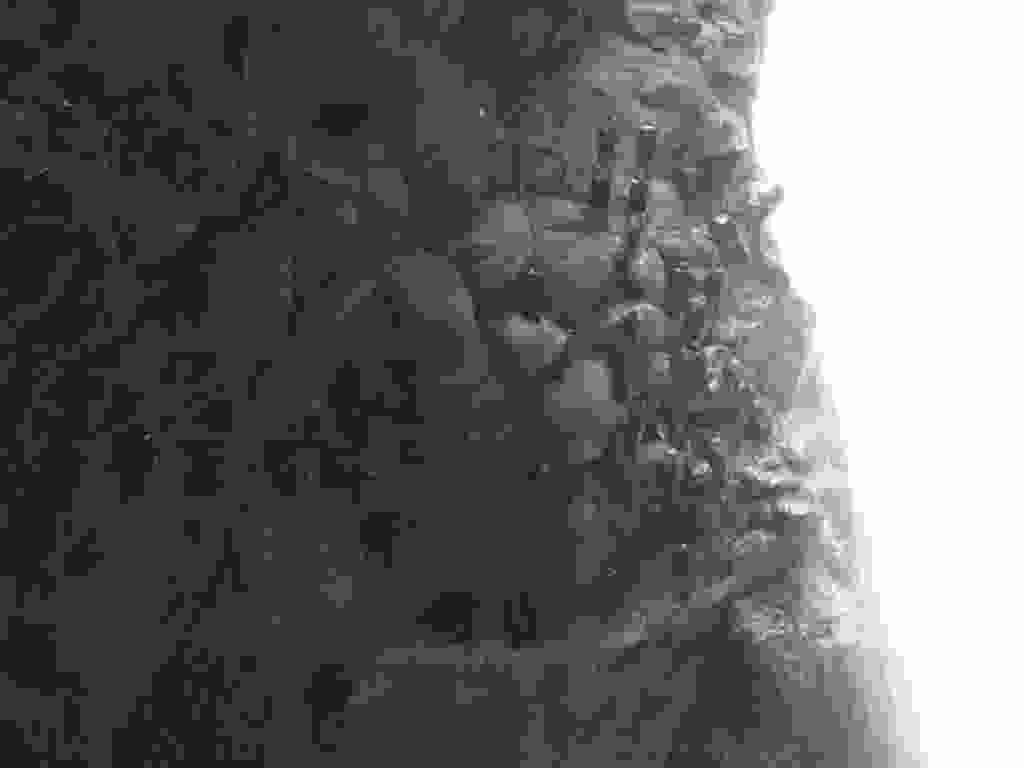
\includegraphics[width=\mywidth]{../wp-content/uploads/2015/06/P6235022-1024x768.jpg} 
\end{center}

Passage par une communauté indigène. 
\begin{center} 
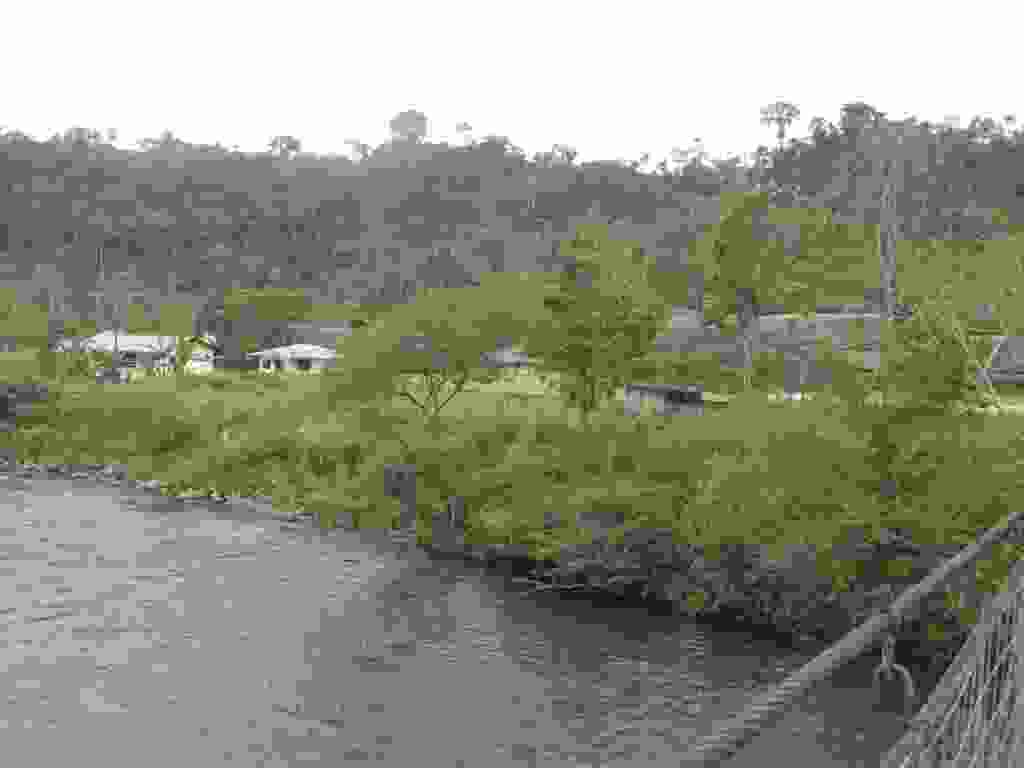
\includegraphics[width=\mywidth]{../wp-content/uploads/2015/06/P6235035-1024x768.jpg} 
\end{center}
\pagebreak

Le temps de se faire peindre le visage avant une balade en barque sur la rivière. 
\begin{center} 
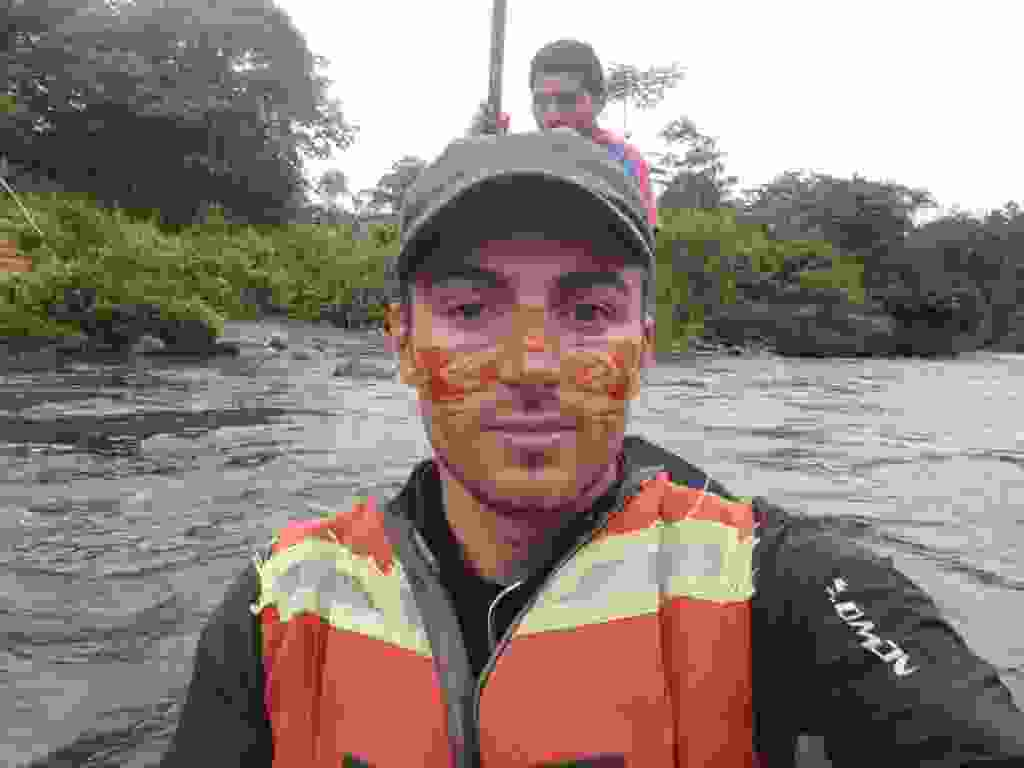
\includegraphics[width=\mywidth]{../wp-content/uploads/2015/06/P6235046-1024x768.jpg} 
\end{center}
\begin{center} 
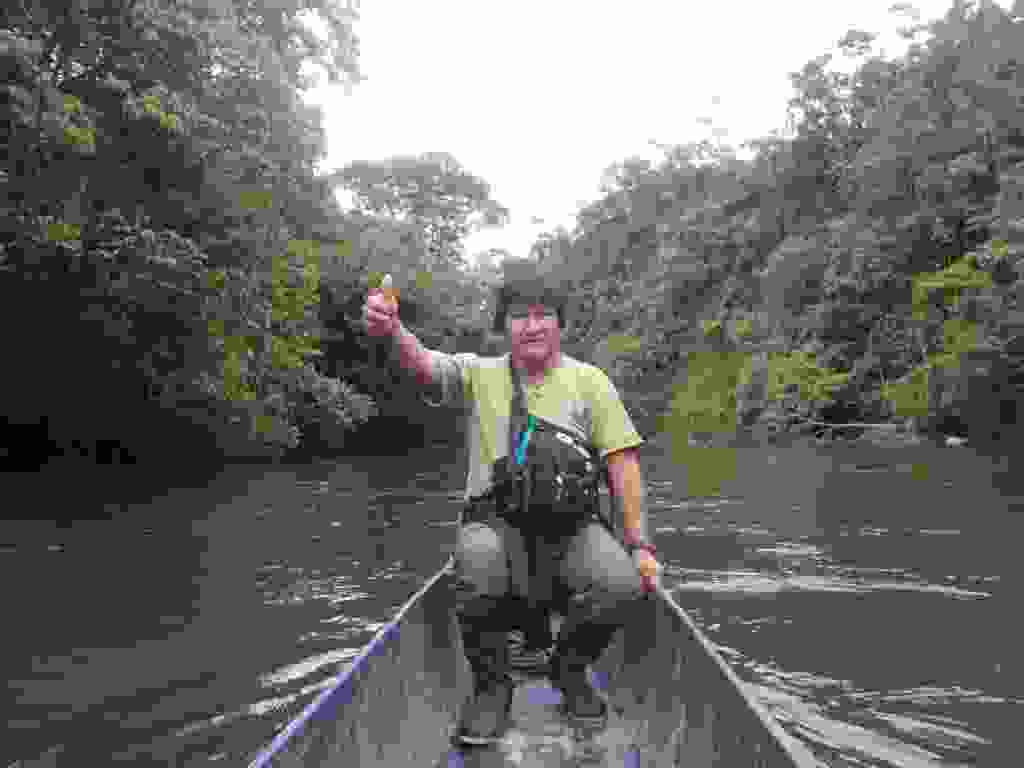
\includegraphics[width=\mywidth]{../wp-content/uploads/2015/06/P6235051-1024x768.jpg} 
\end{center}

\pagebreak
Mirador sur la jungle. 
\begin{center} 
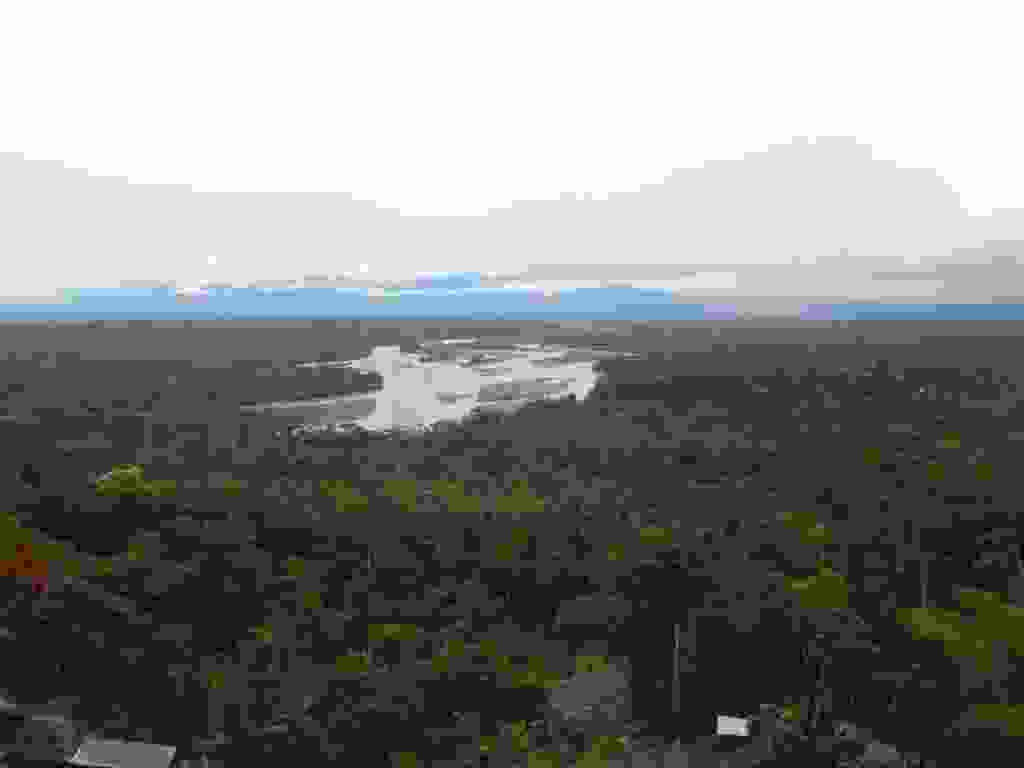
\includegraphics[width=\mywidth]{../wp-content/uploads/2015/06/P6235060-1024x768.jpg} 
\end{center}

Des ananas sur le chemin. 
\begin{center} 
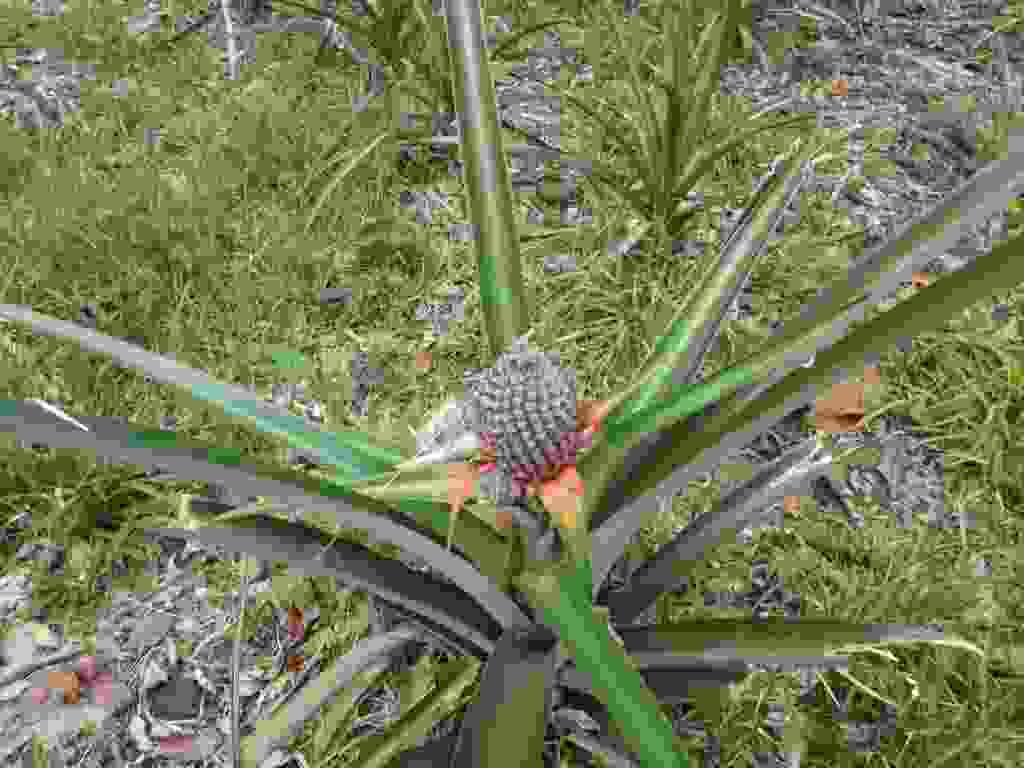
\includegraphics[width=\mywidth]{../wp-content/uploads/2015/06/P6235063-1024x768.jpg} 
\end{center}
\pagebreak

Le lac aux crocodiles. 
\begin{center} 
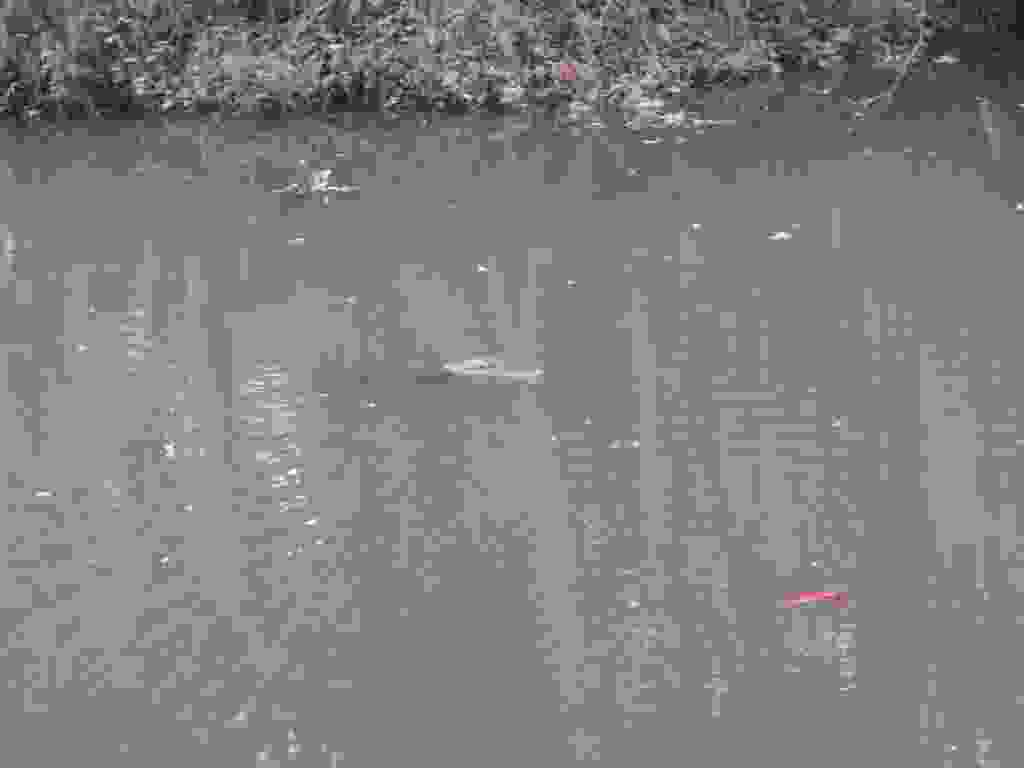
\includegraphics[width=\mywidth]{../wp-content/uploads/2015/06/P6235070-1024x768.jpg} 
\end{center}

La journée se termine dans la propriété familiale de Enrique ou j'assiste à la fabrication de meubles artisanaux. 
\begin{center} 
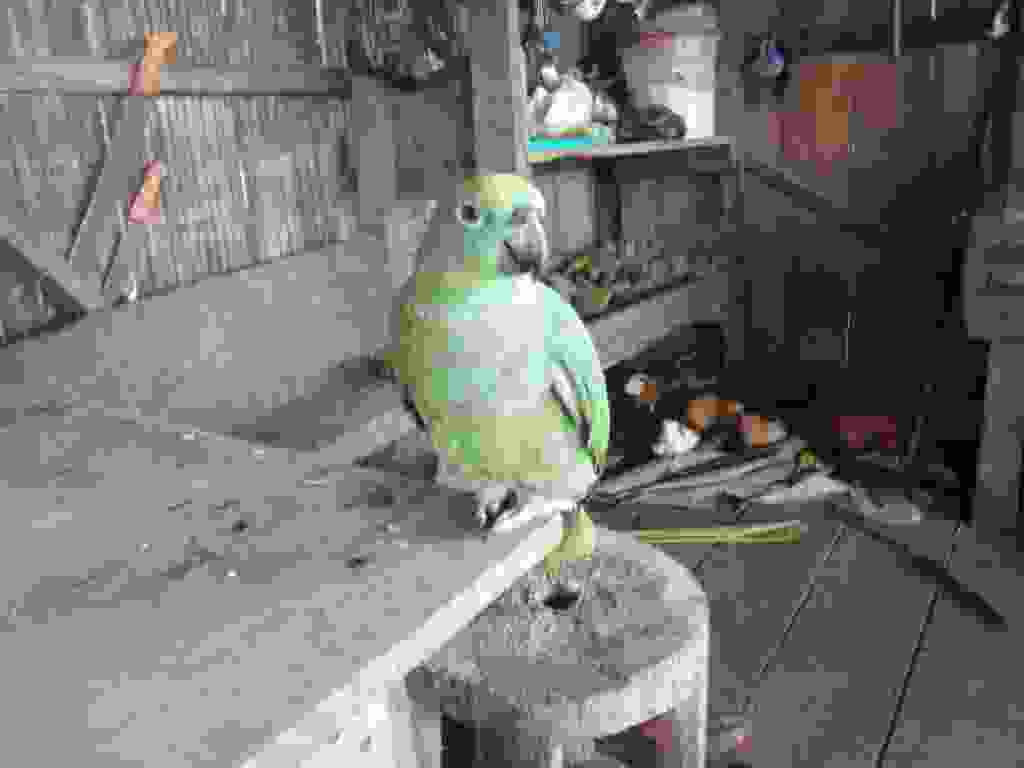
\includegraphics[width=\mywidth]{../wp-content/uploads/2015/06/P6235074-1024x768.jpg} 
\end{center}
\begin{center} 
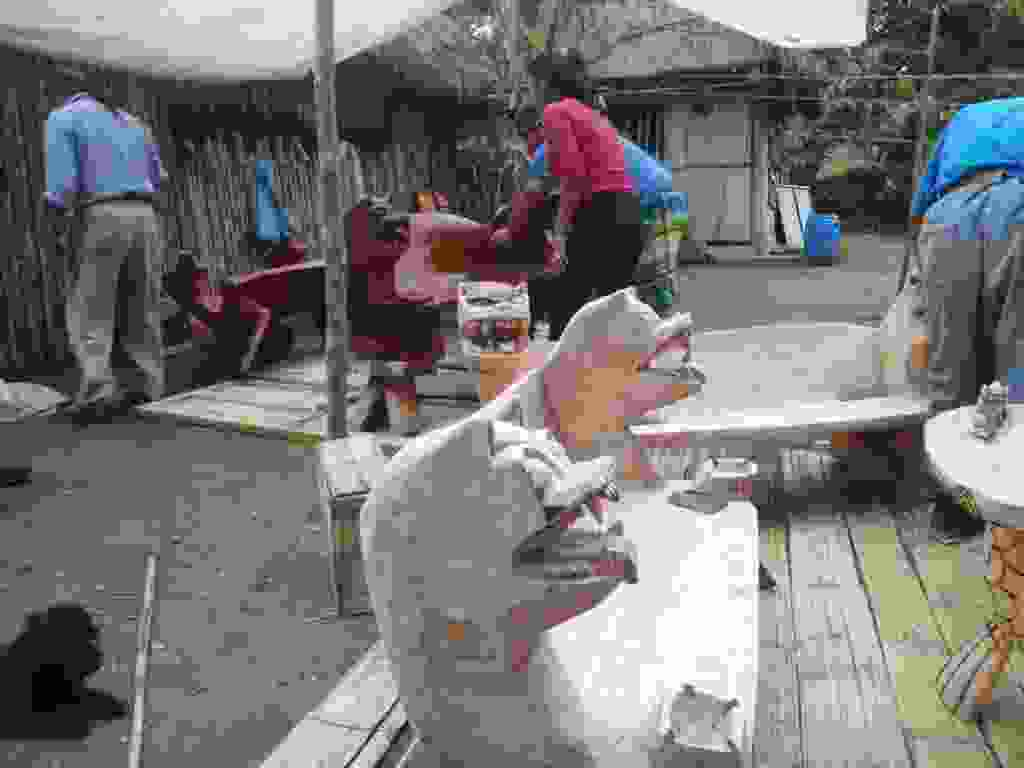
\includegraphics[width=\mywidth]{../wp-content/uploads/2015/06/P6235077-1024x768.jpg} 
\end{center}

Je remonte ensuite sur la route vers Quito. 
\begin{center} 
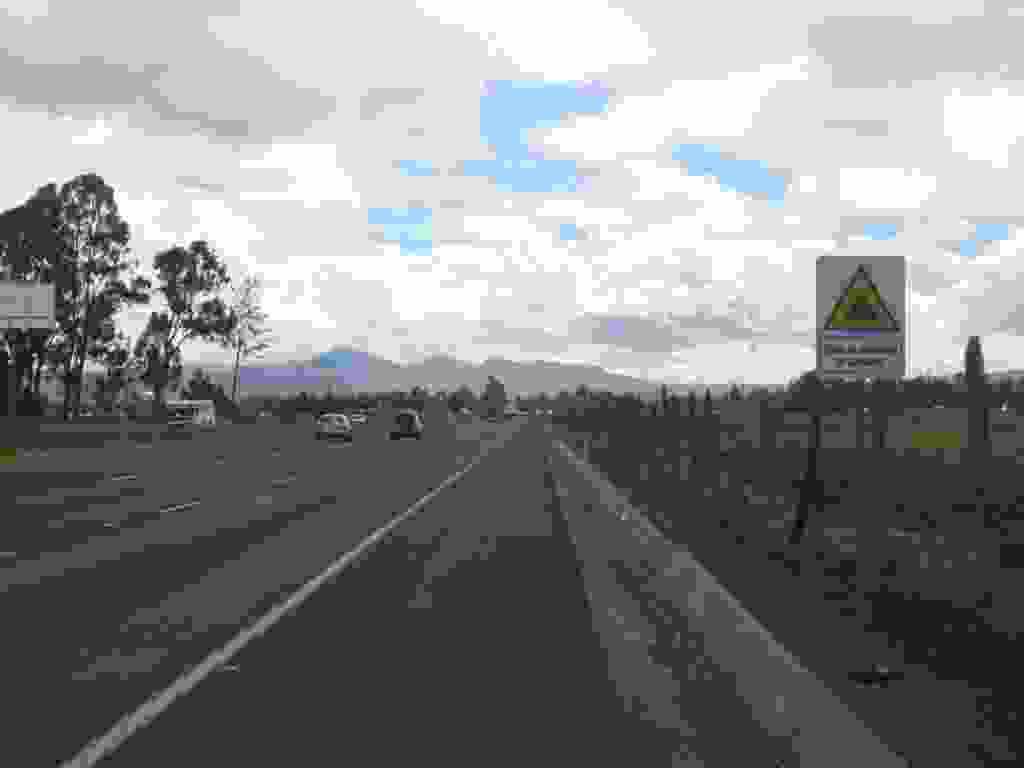
\includegraphics[width=\mywidth]{../wp-content/uploads/2015/06/P6255087-1024x768.jpg} 
\end{center}
\pagebreak

Je fais étape a Latacunga, pour une sympathique soirée chez Javier et sa famille. 
\begin{center} 
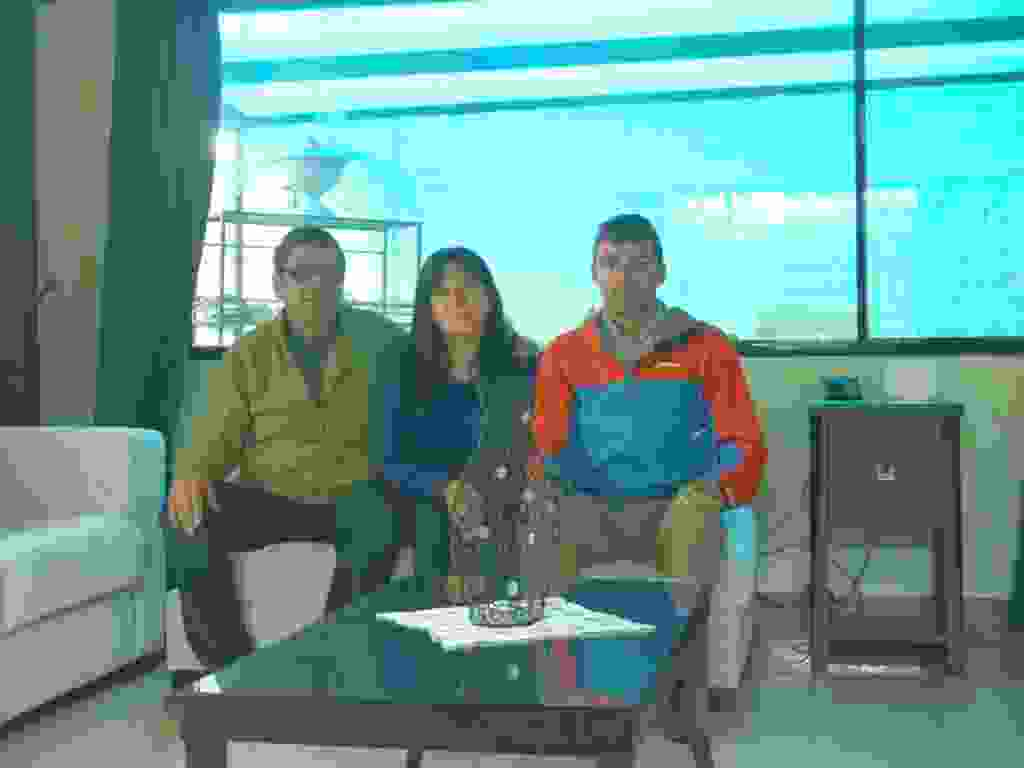
\includegraphics[width=\mywidth]{../wp-content/uploads/2015/06/P6255084-1024x768.jpg} 
\end{center}

La route me mène dans le parc national Cotopaxi. 
\begin{center} 
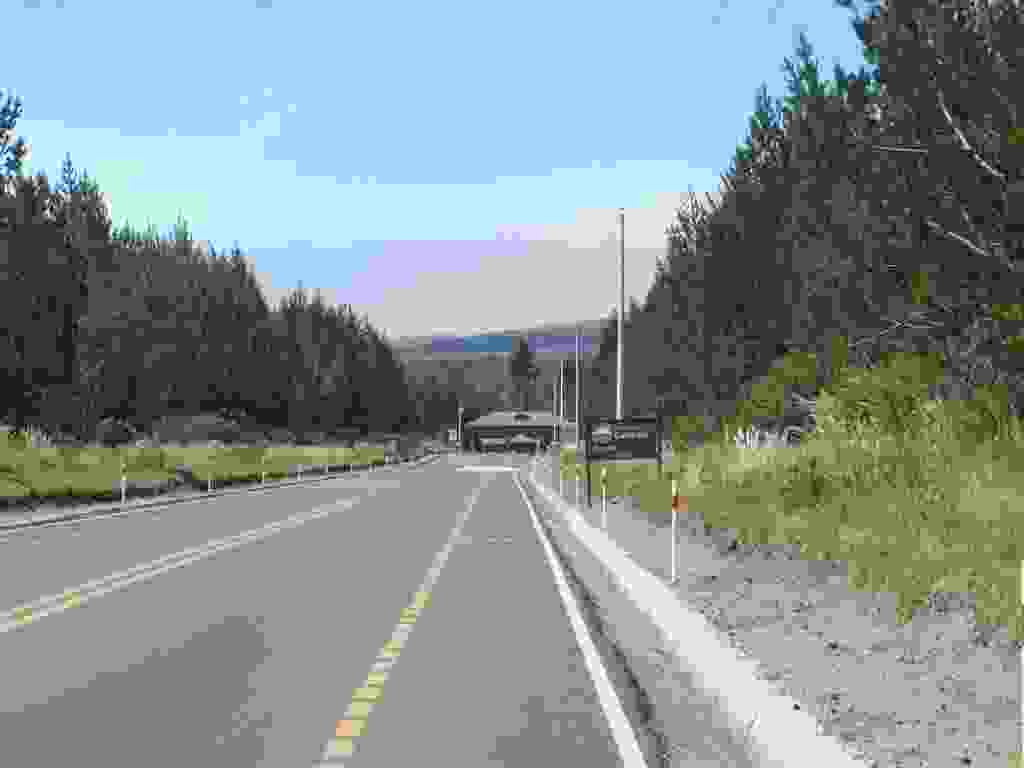
\includegraphics[width=\mywidth]{../wp-content/uploads/2015/06/P6255095-1024x768.jpg} 
\end{center}
\pagebreak

Le Cotopaxi est un volcan actif qui culmine à 5800m. 
\begin{center} 
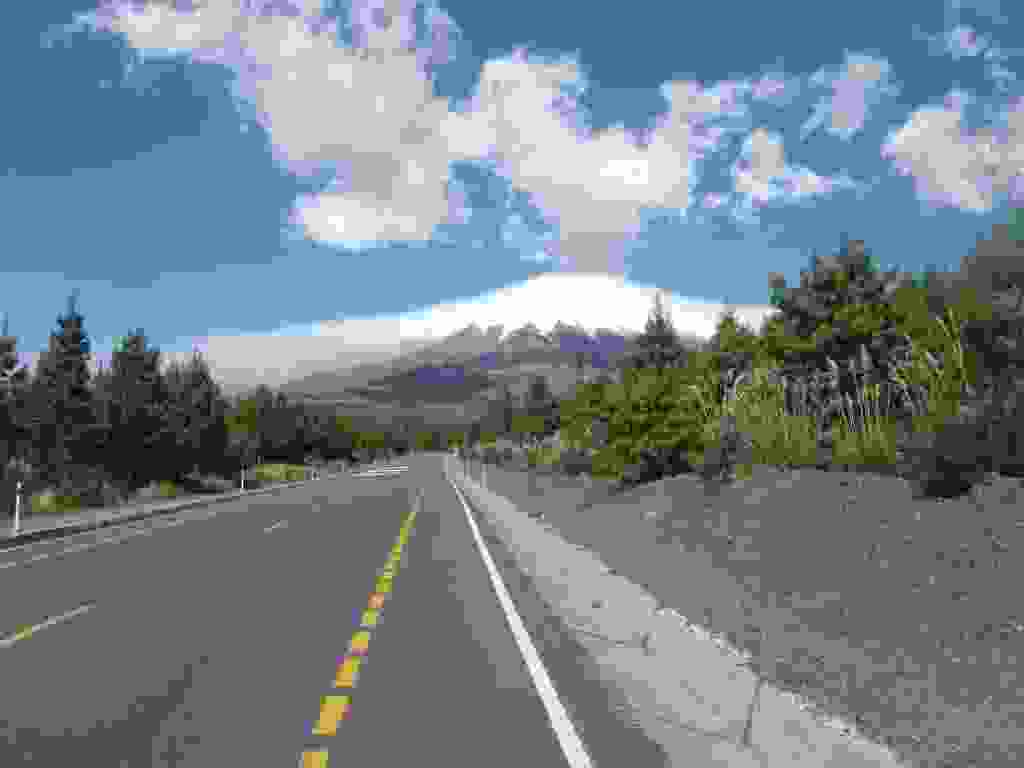
\includegraphics[width=\mywidth]{../wp-content/uploads/2015/06/P6255097-1024x768.jpg} 
\end{center}
\begin{center} 
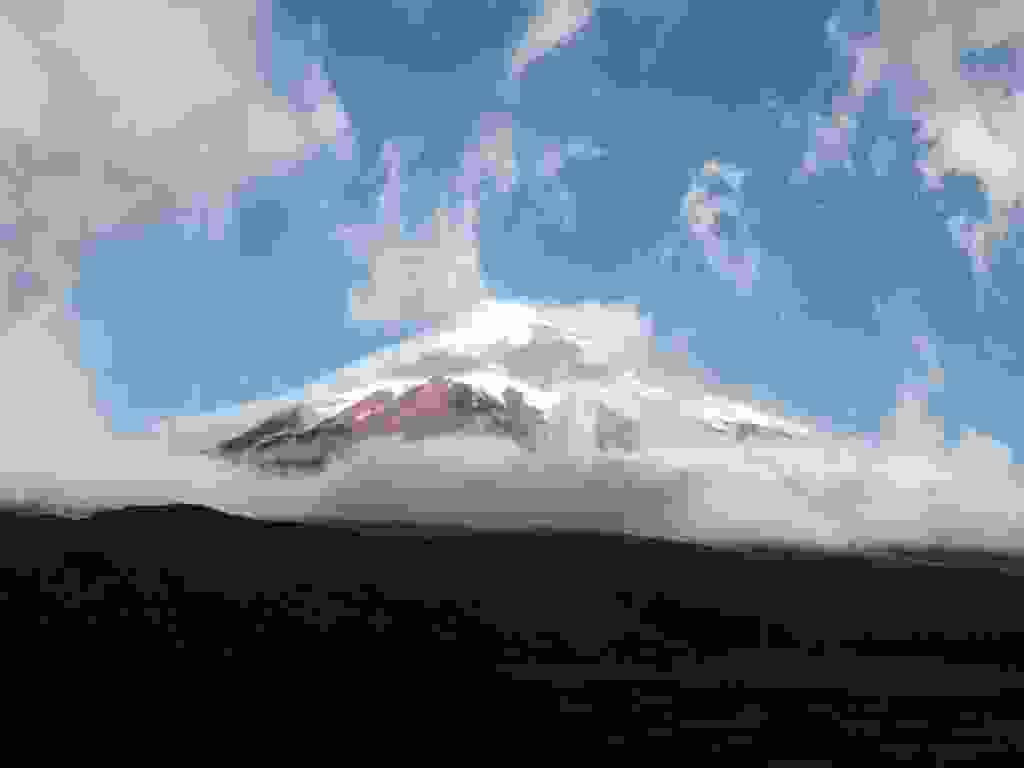
\includegraphics[width=\mywidth]{../wp-content/uploads/2015/06/P6265107-1024x768.jpg} 
\end{center}
\pagebreak

Je passe la nuit dans le camping du parc, pas d'autres campeurs ce jour là. 
\begin{center} 
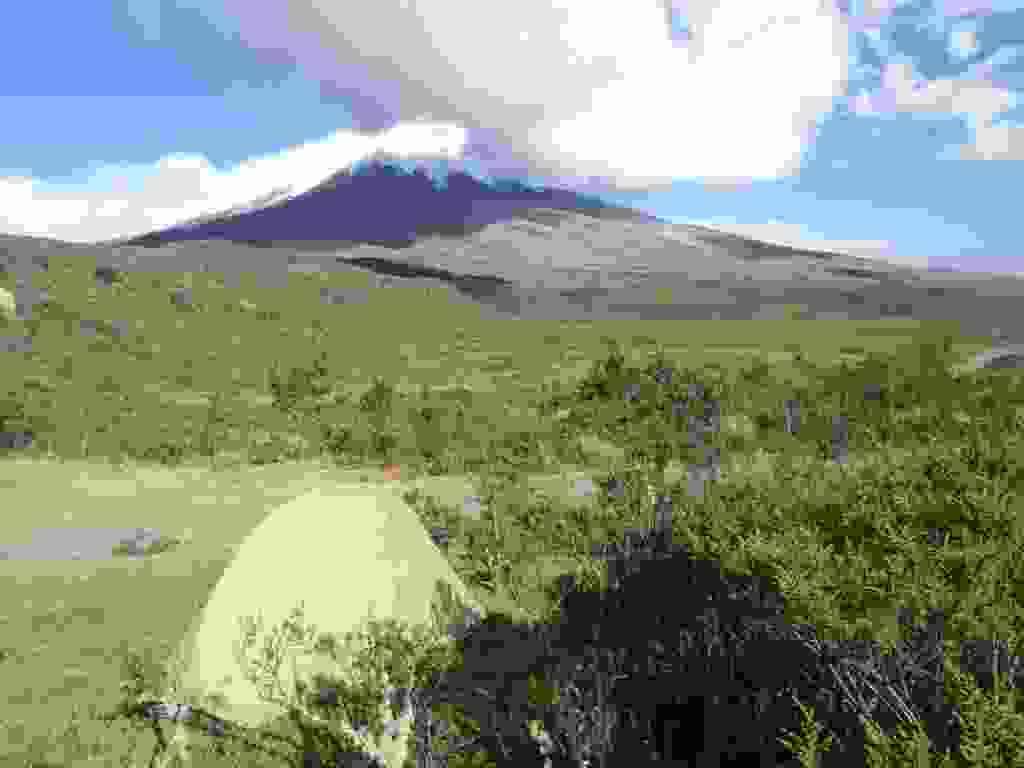
\includegraphics[width=\mywidth]{../wp-content/uploads/2015/06/P6255104-1024x768.jpg} 
\end{center}

Le lendemain je monte à la Laguna Limpiopungo à 3800m. 
\begin{center} 
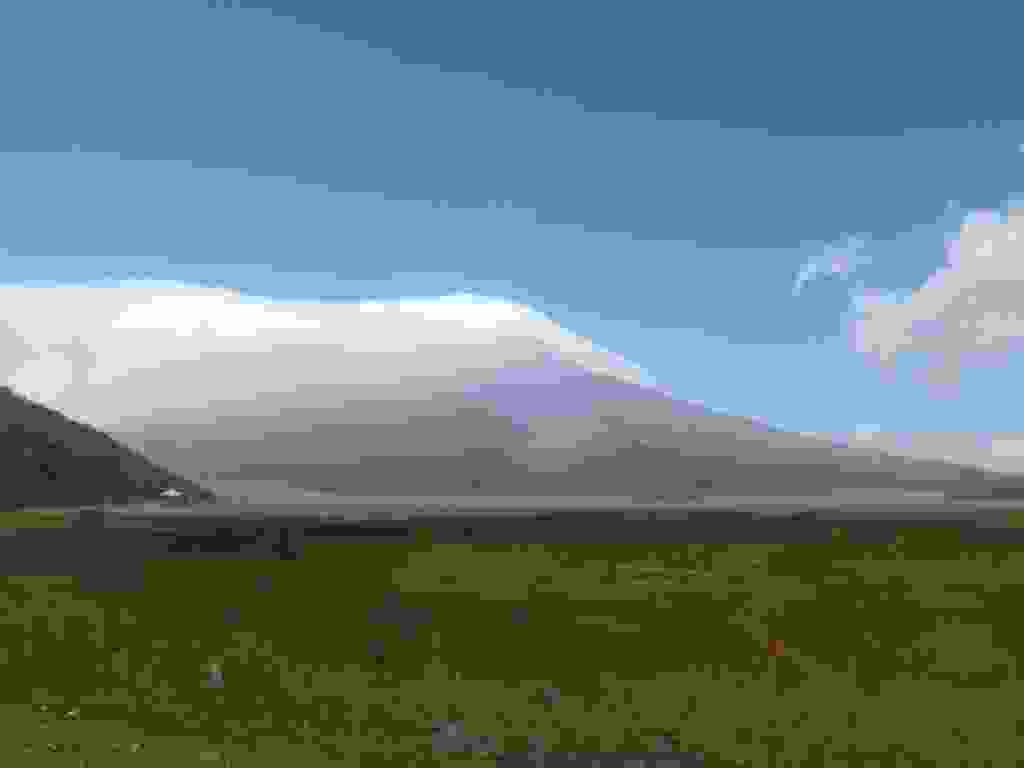
\includegraphics[width=\mywidth]{../wp-content/uploads/2015/06/P6265111-1024x768.jpg} 
\end{center}
\pagebreak

Là haut le vent est très fort et m'empêche de continuer plus loin. Je reviens donc sur la route principale vers Quito. 
\begin{center}
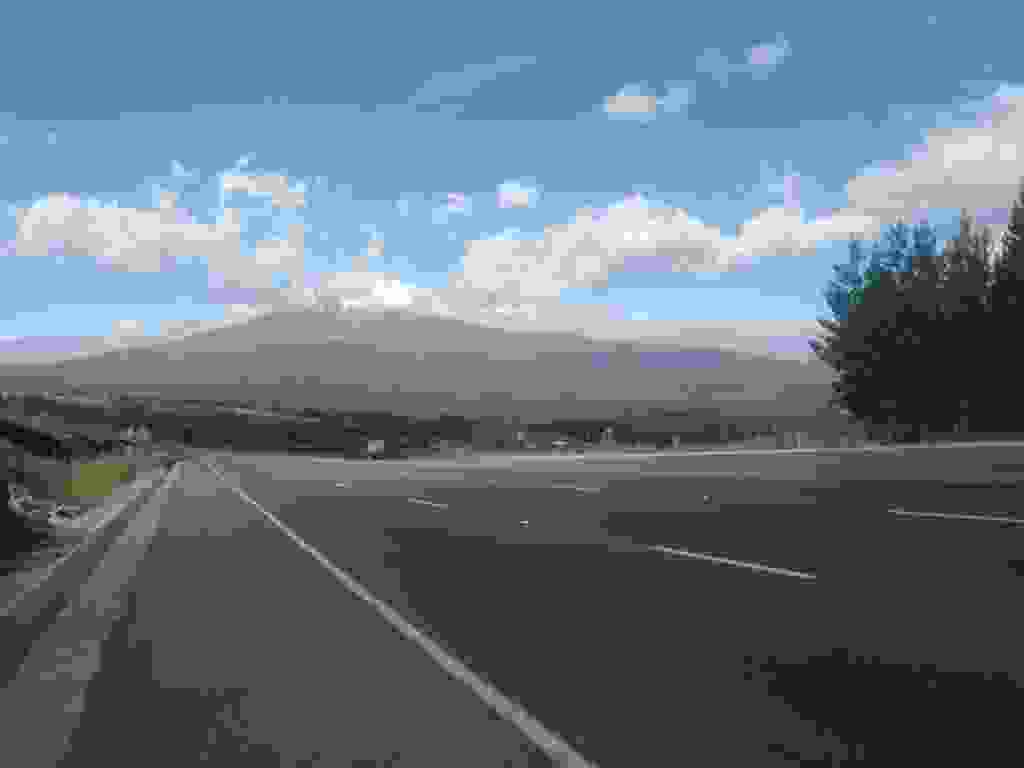
\includegraphics[width=\mywidth]{../wp-content/uploads/2015/06/P6265115-1024x768.jpg} 
\end{center}

J'arrive à Sangolqui, ville de la banlieue ou je suis hébergé par Pablo et sa famille : un accueil excellent ! 
\begin{center} 
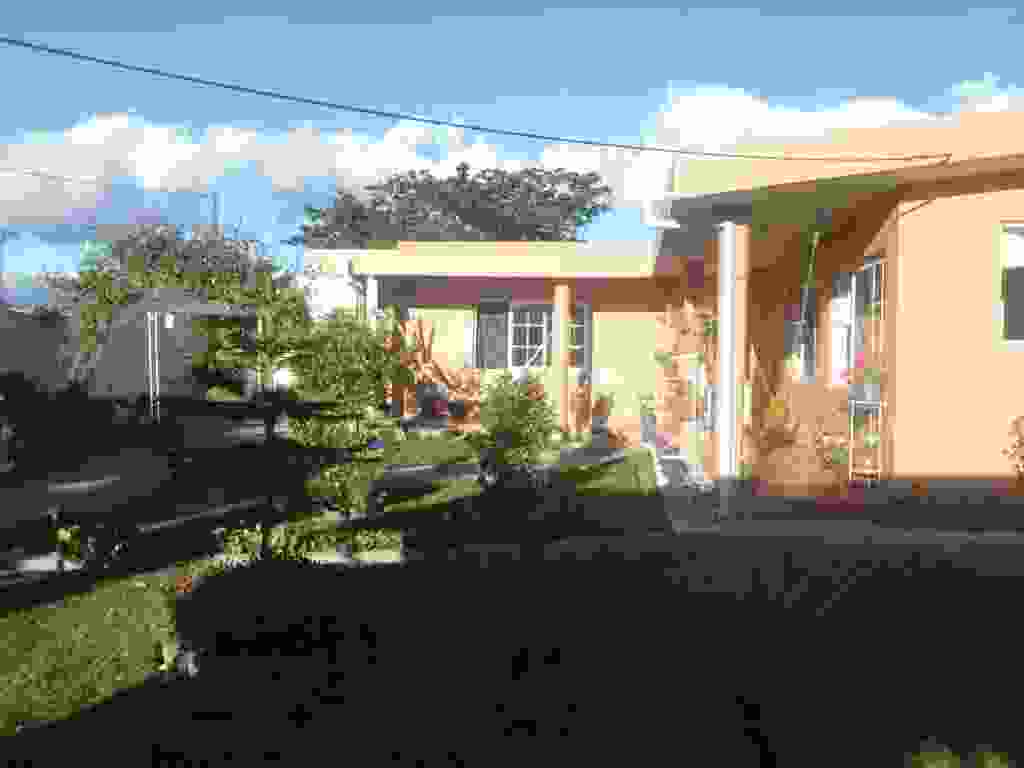
\includegraphics[width=\mywidth]{../wp-content/uploads/2015/06/P6275118-1024x768.jpg} 
\end{center}
\begin{center}
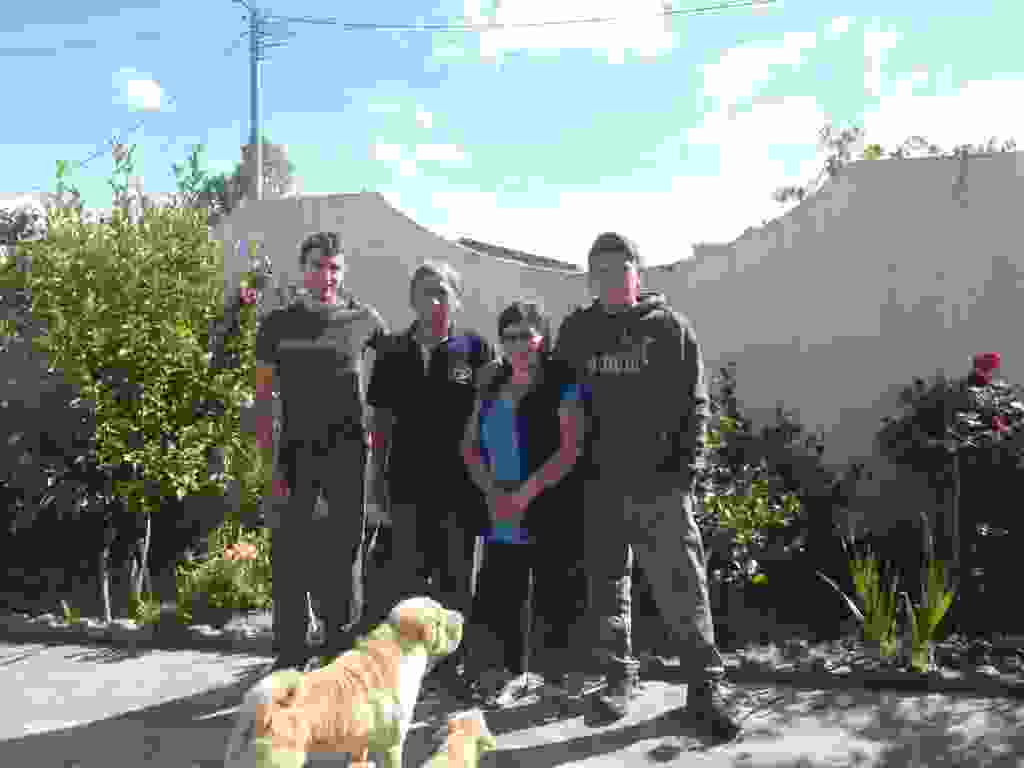
\includegraphics[width=\mywidth]{../wp-content/uploads/2015/06/P6295144-1024x768.jpg} 
\end{center}

Balade sur une petite montagne proche avec Pablo et un cousin. 
\begin{center} 
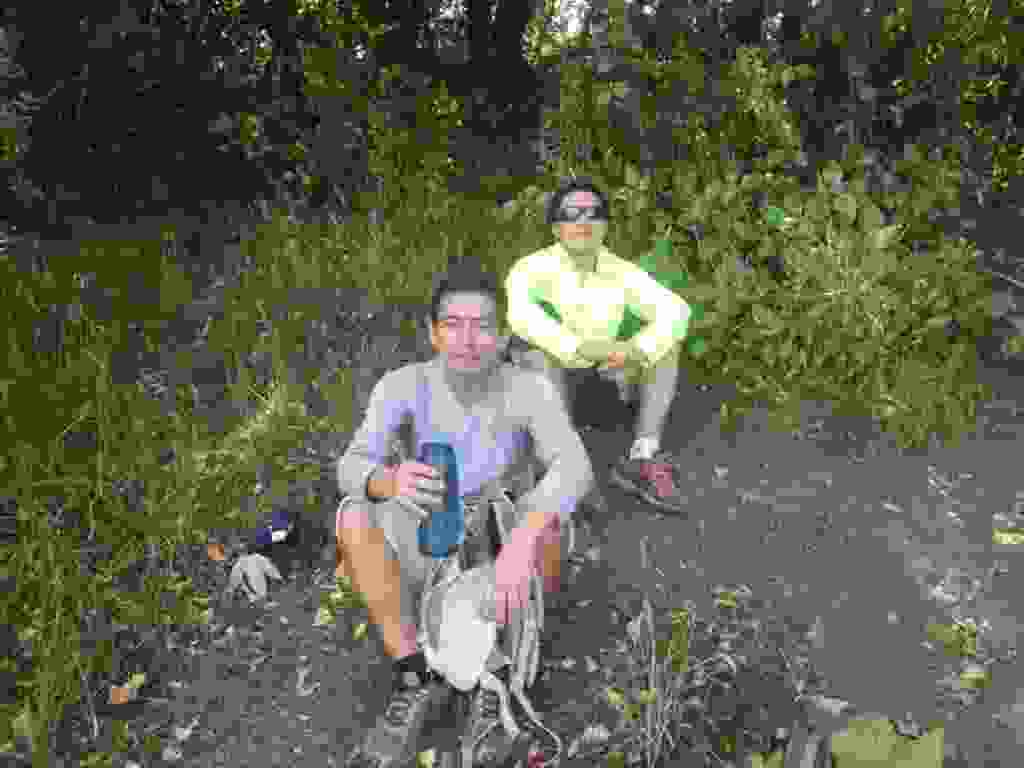
\includegraphics[width=\mywidth]{../wp-content/uploads/2015/06/P6285136-1024x768.jpg} 
\end{center}
\begin{center} 
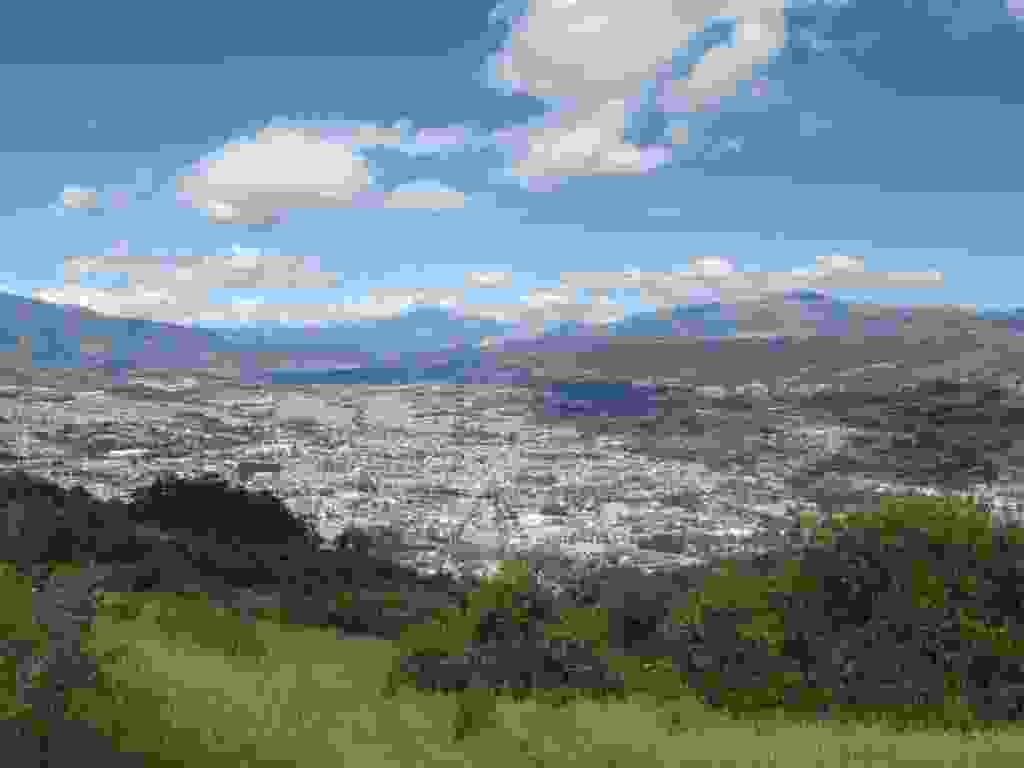
\includegraphics[width=\mywidth]{../wp-content/uploads/2015/06/P6285132-1024x768.jpg} 
\end{center}
\begin{center} 
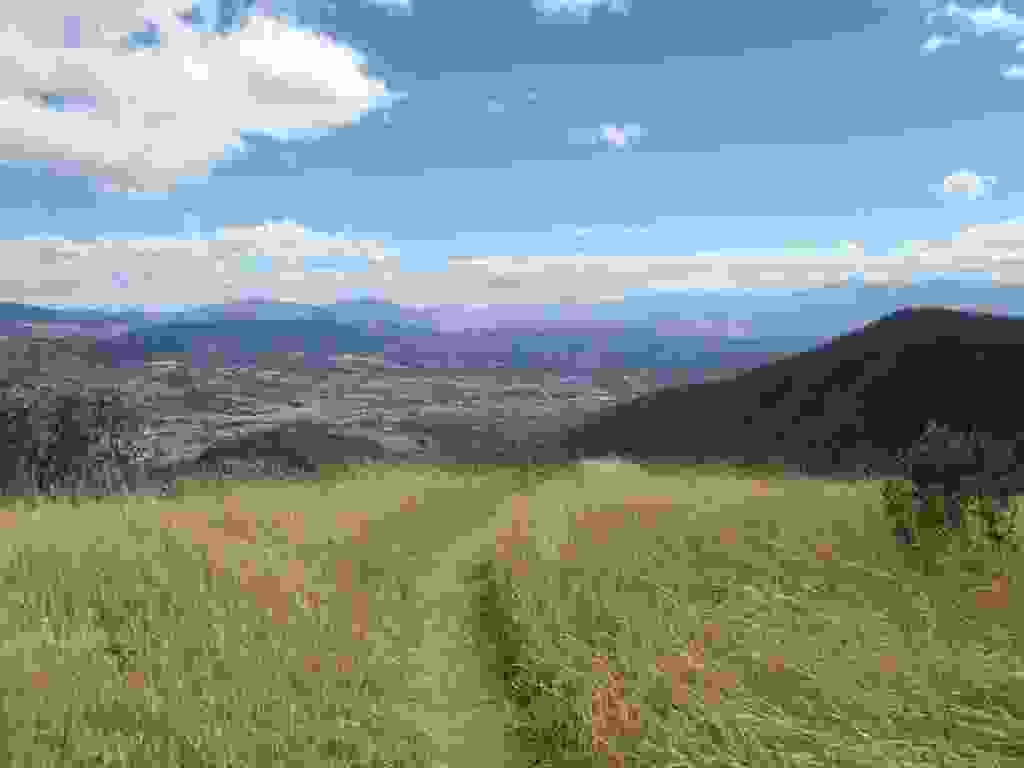
\includegraphics[width=\mywidth]{../wp-content/uploads/2015/06/P6285140-1024x768.jpg} 
\end{center}
\pagebreak

Je visite le centre historique de Quito. 
\begin{center} 
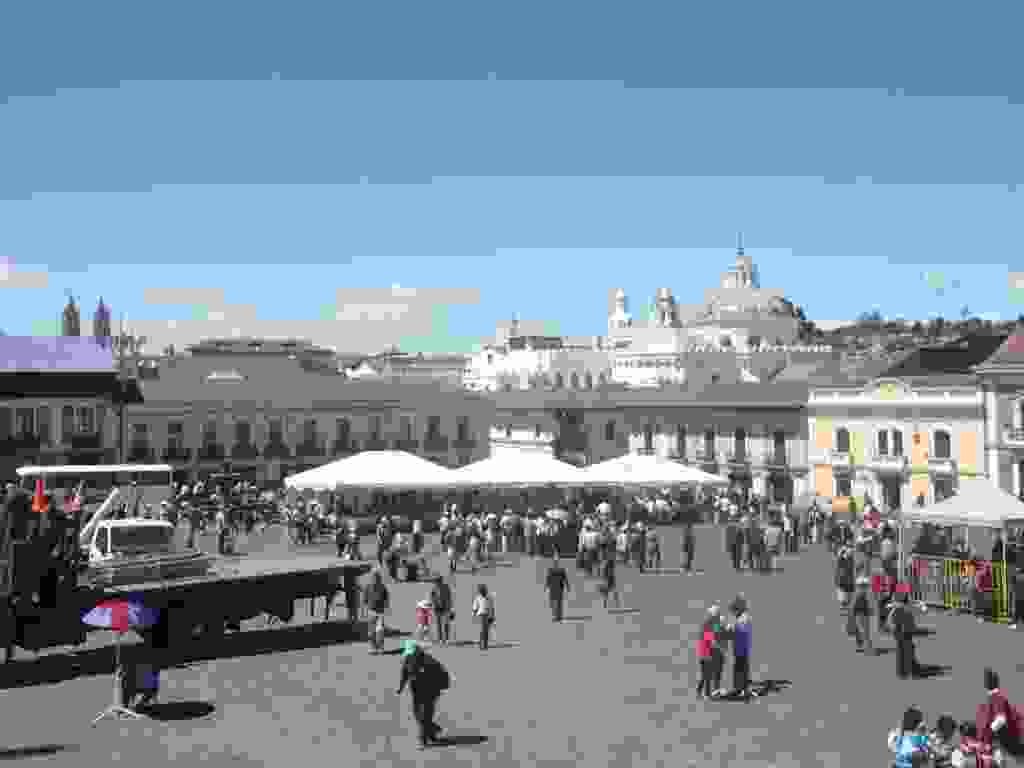
\includegraphics[width=\mywidth]{../wp-content/uploads/2015/06/P6275127-1024x768.jpg} 
\end{center}
\begin{center} 
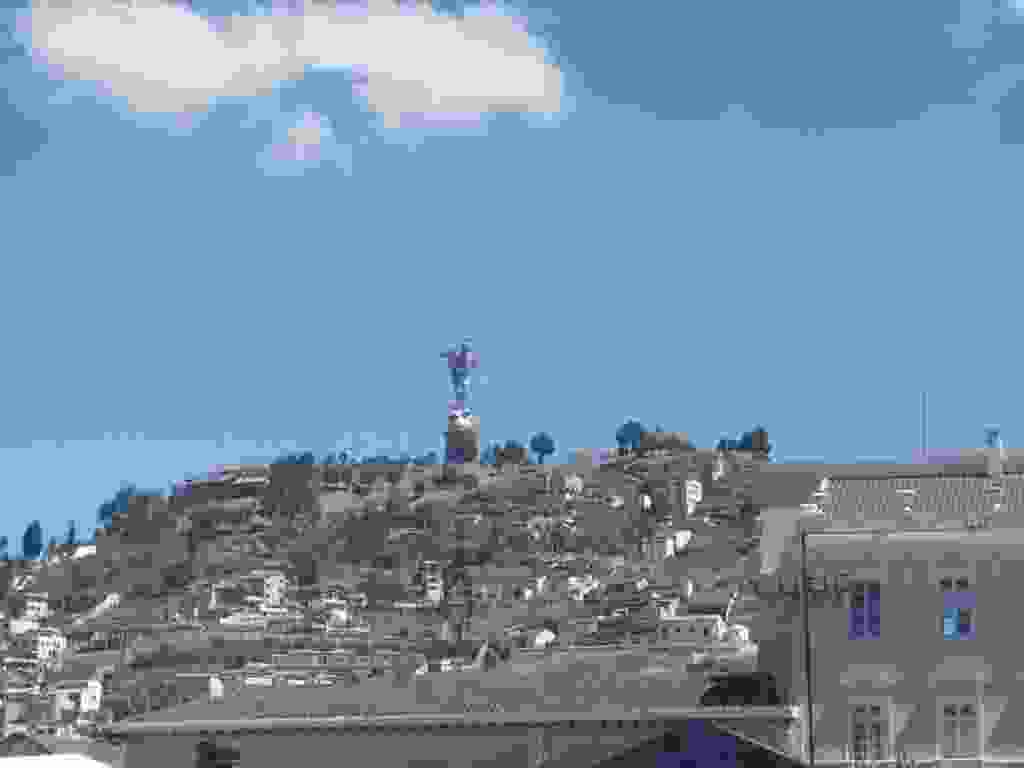
\includegraphics[width=\mywidth]{../wp-content/uploads/2015/06/P6275128-1024x768.jpg} 
\end{center}
\begin{center} 
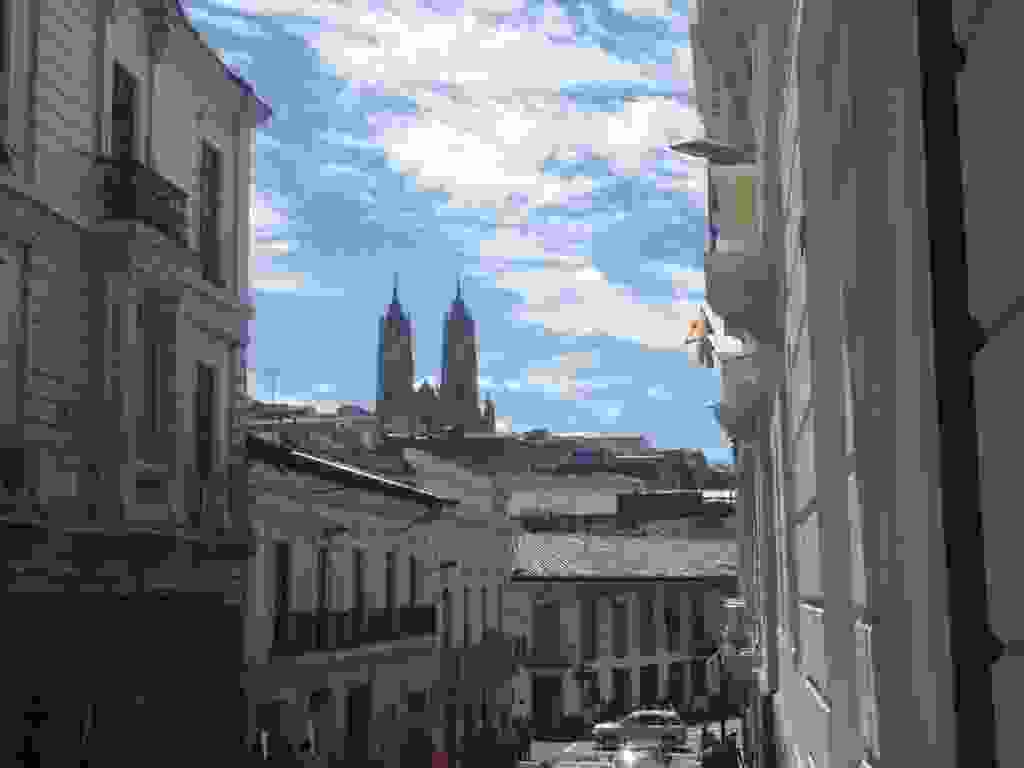
\includegraphics[width=\mywidth]{../wp-content/uploads/2015/06/P6305155-1024x768.jpg} 
\end{center}
\begin{center} 
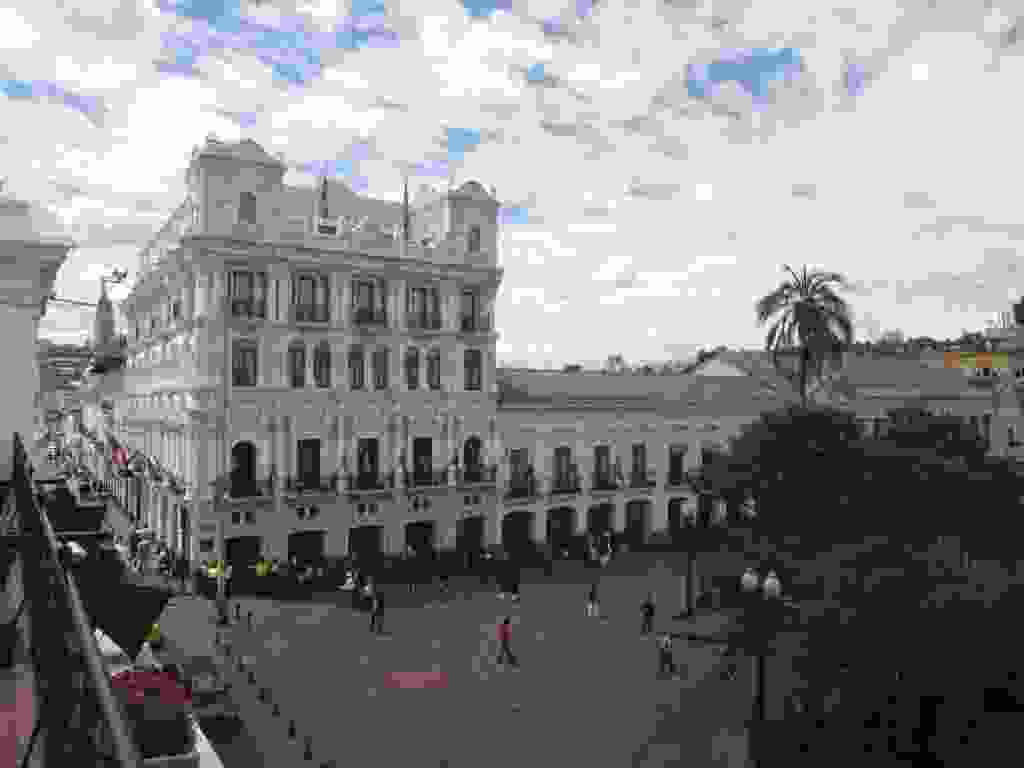
\includegraphics[width=\mywidth]{../wp-content/uploads/2015/06/P6305170-1024x768.jpg} 
\end{center}
\begin{center} 
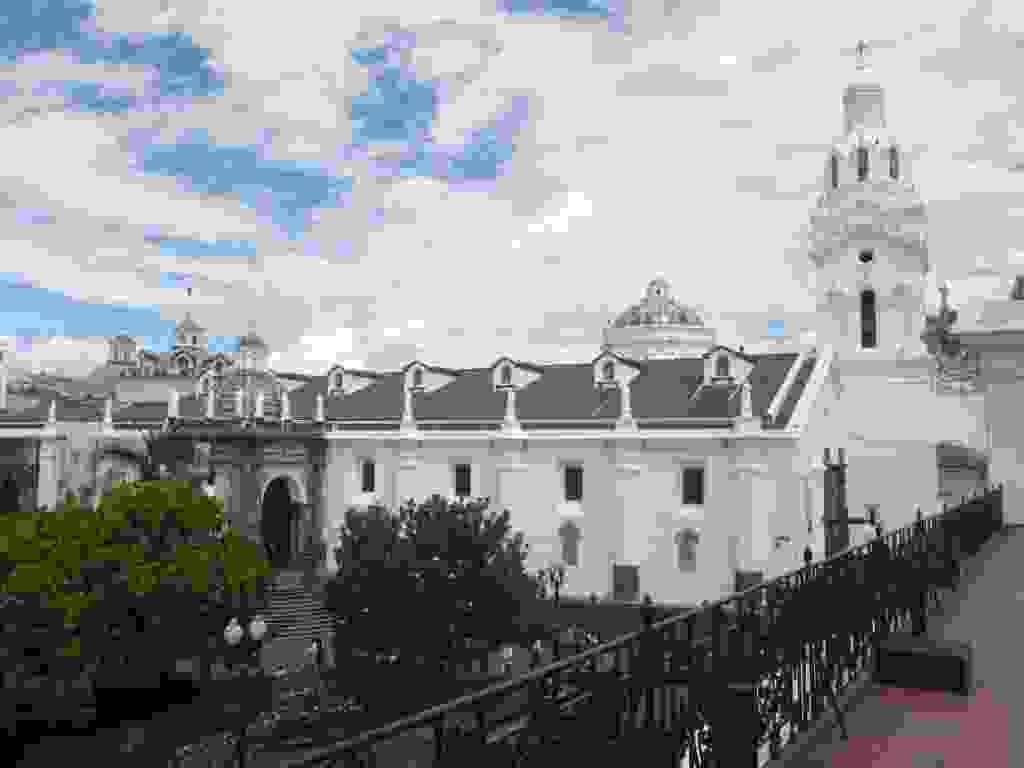
\includegraphics[width=\mywidth]{../wp-content/uploads/2015/06/P6305171-1024x768.jpg} 
\end{center}

Il y a des dizaines, peut être des centaines d'églises. 
\begin{center} 
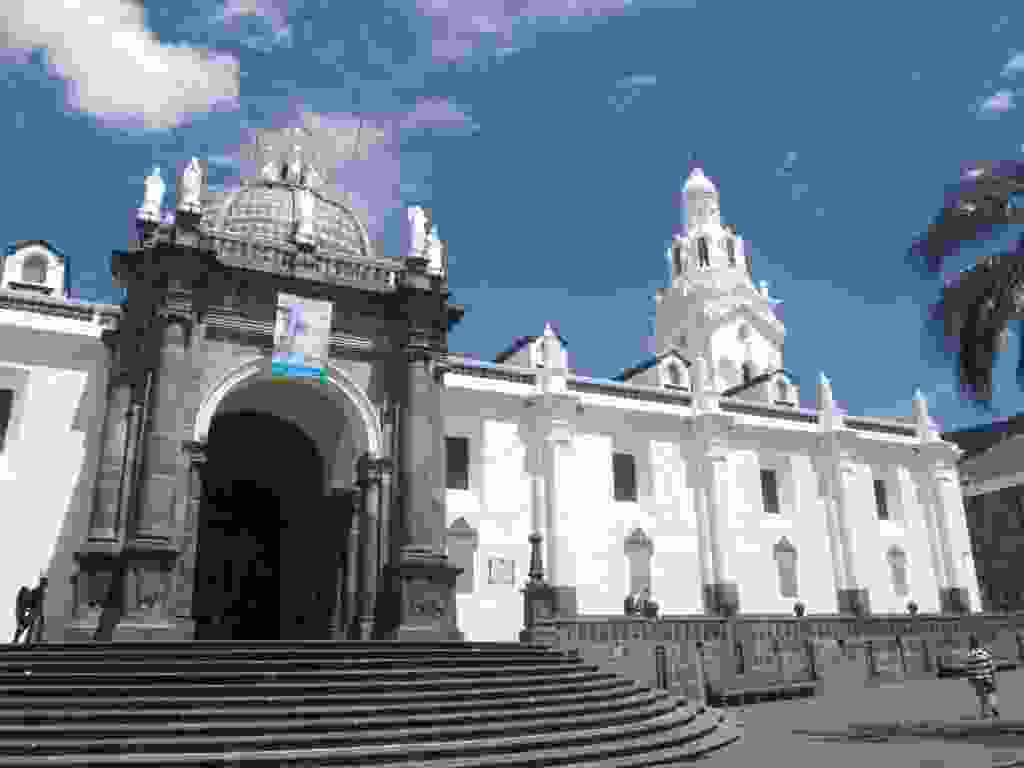
\includegraphics[width=\mywidth]{../wp-content/uploads/2015/06/P6305161-1024x768.jpg}
\end{center}
\pagebreak

L'église Compania de Jesus dont l'intérieur est recouvert d'or. 
\begin{center} 
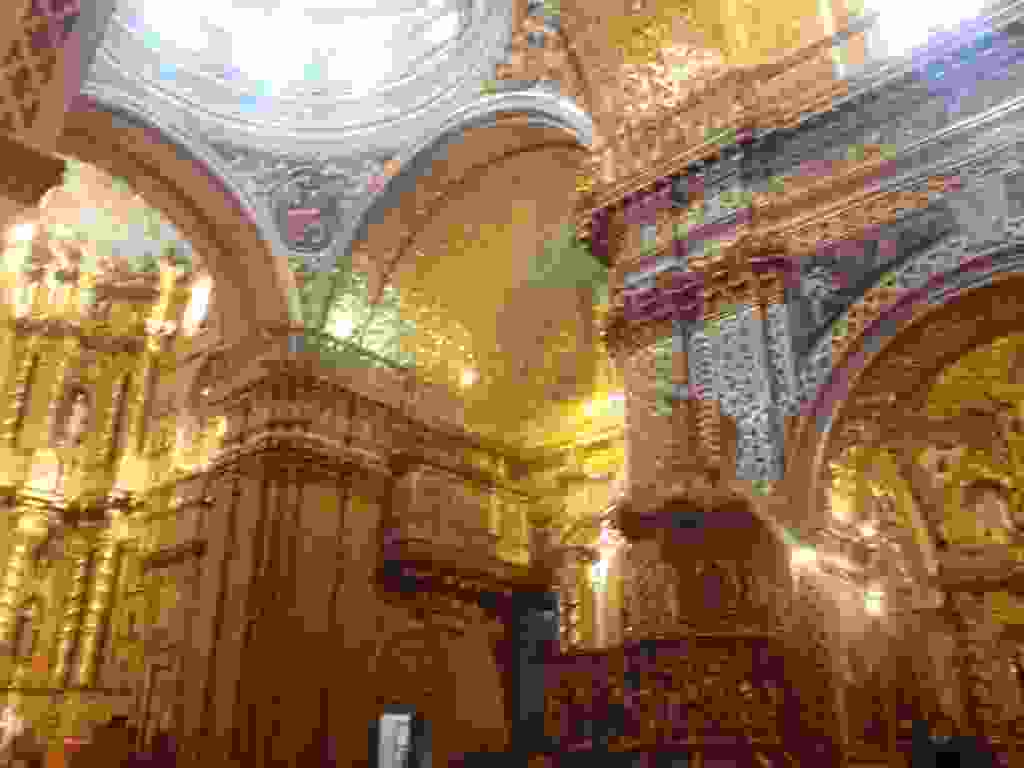
\includegraphics[width=\mywidth]{../wp-content/uploads/2015/06/P6275121-1024x768.jpg} 
\end{center}

La basilique gothique. 
\begin{center} 
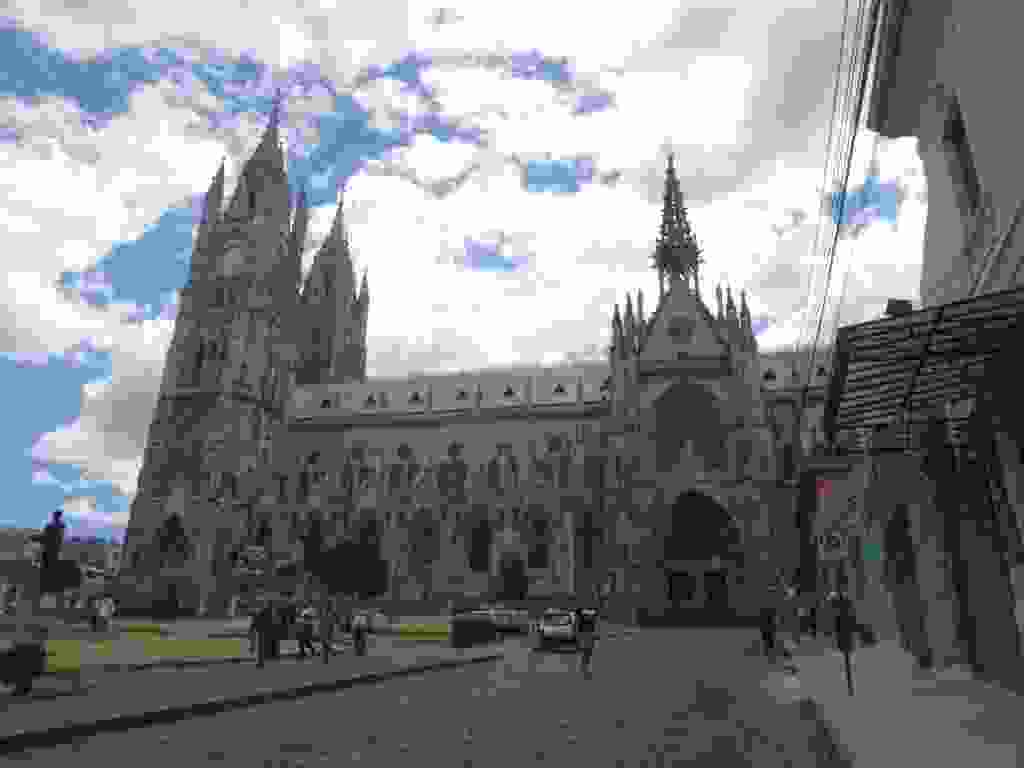
\includegraphics[width=\mywidth]{../wp-content/uploads/2015/06/P6305185-1024x768.jpg} 
\end{center}

\pagebreak

Le palais présidentiel ouvert au public gratuitement. 
\begin{center} 
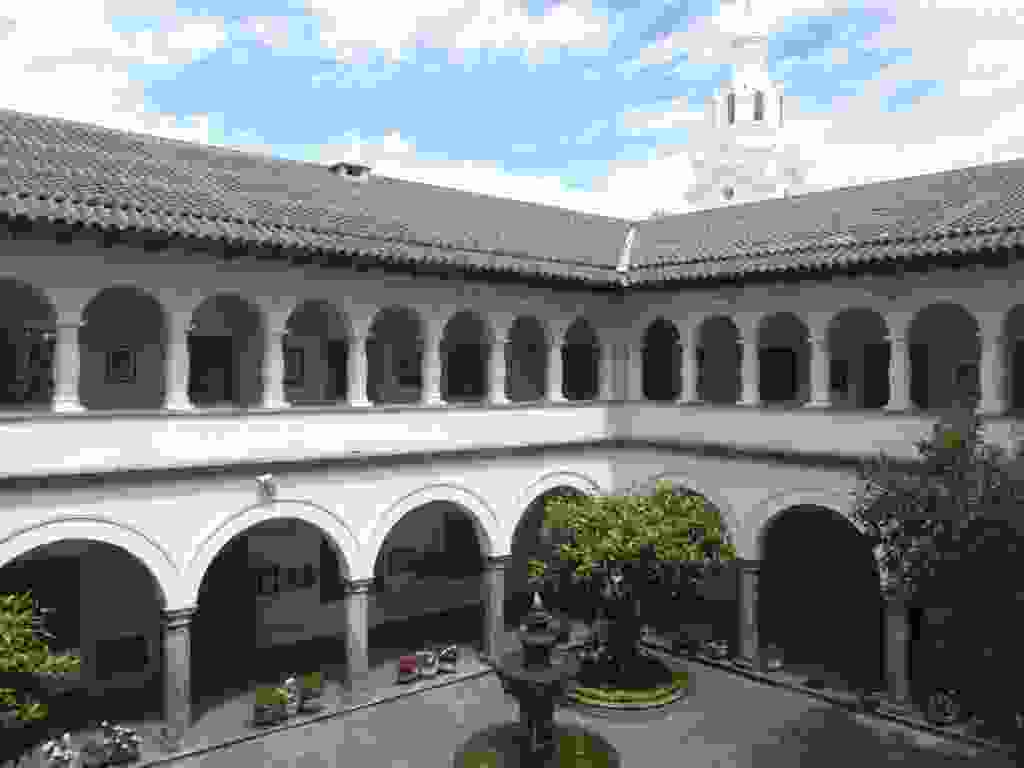
\includegraphics[width=\mywidth]{../wp-content/uploads/2015/06/P6305183-1024x768.jpg} 
\end{center}

On peut visiter différentes salles et voir les cadeaux fait au président équatorien par des présidents étrangers. 
\begin{center} 
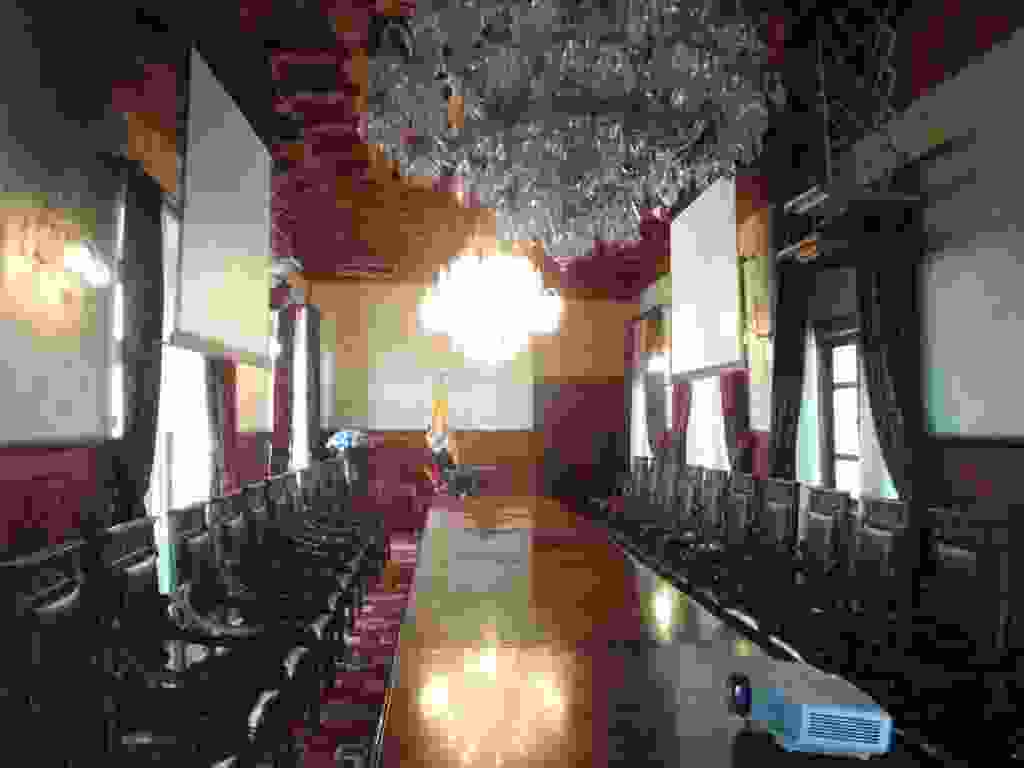
\includegraphics[width=\mywidth]{../wp-content/uploads/2015/06/P6305168-1024x768.jpg} 
\end{center}
\begin{center} 
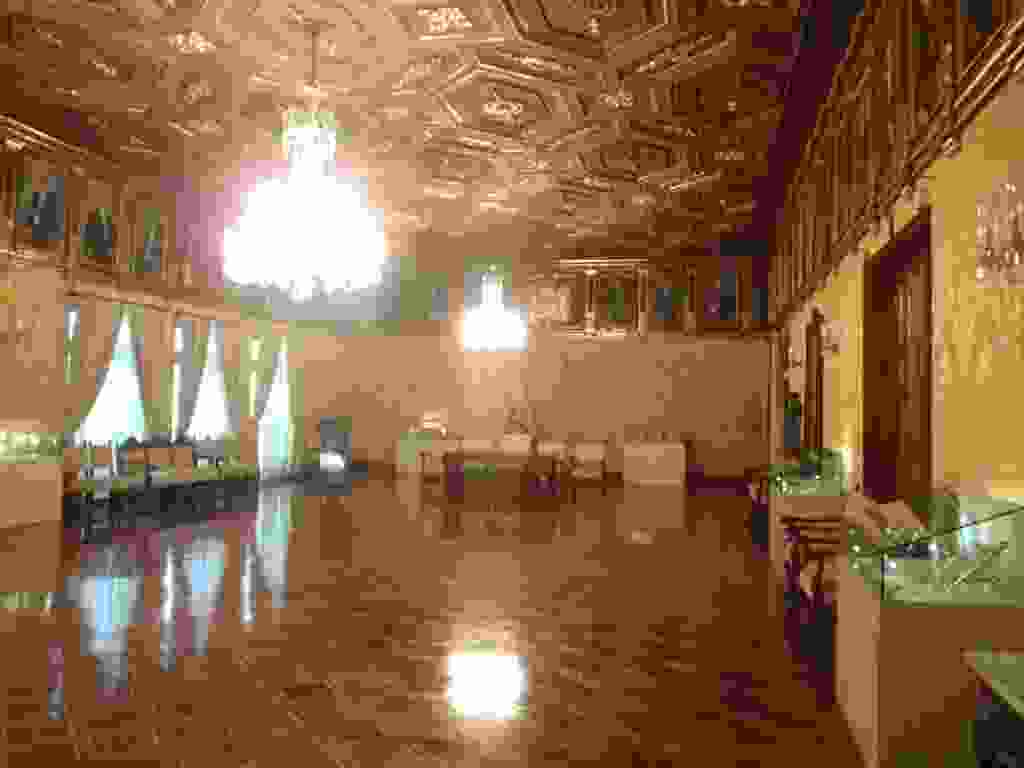
\includegraphics[width=\mywidth]{../wp-content/uploads/2015/06/P6305179-1024x768.jpg} 
\end{center}
\begin{center} 
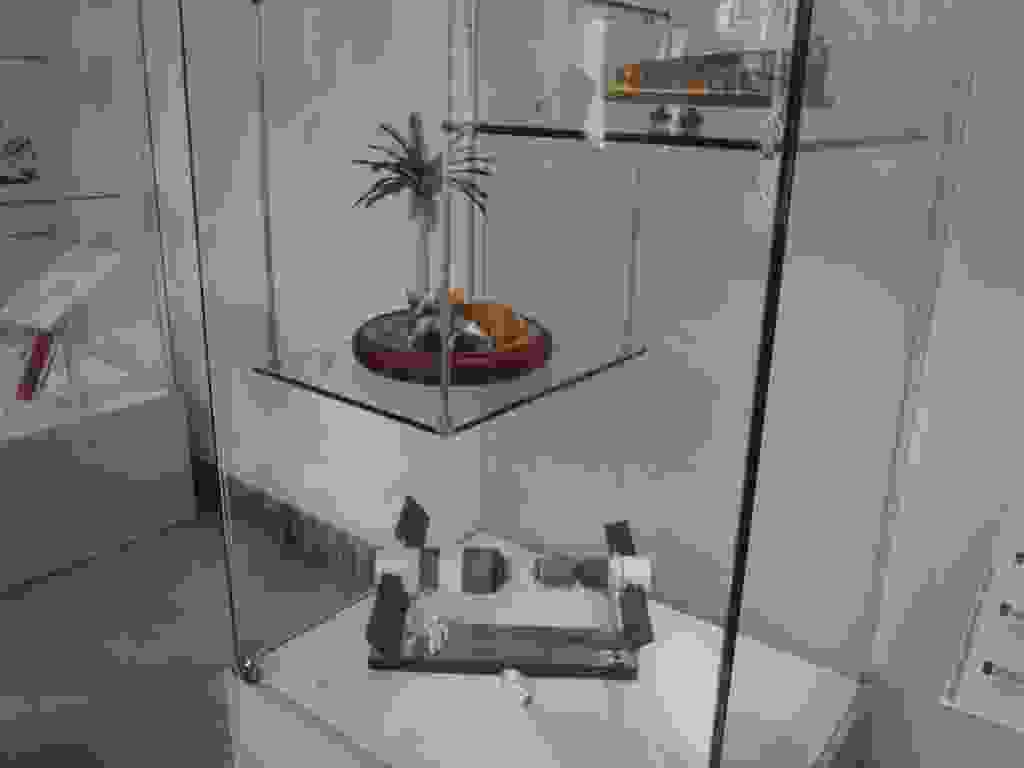
\includegraphics[width=\mywidth]{../wp-content/uploads/2015/06/P6305177-1024x768.jpg} 
\end{center}
\pagebreak

Avant de m'envoler vers les Galapagos, j'ai passé deux jours dans une ferme à Pifo, un village près de Quito.  Quatre familles s'y sont regroupées pour faire de l'élevage et du maraichage.
\begin{center} 
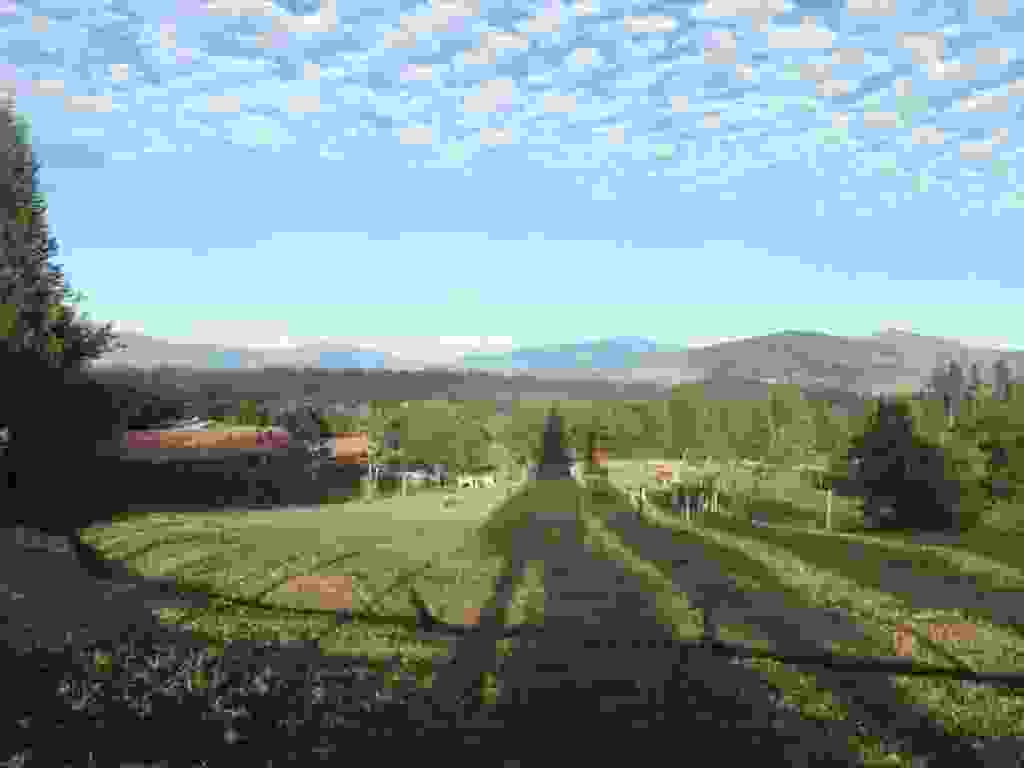
\includegraphics[width=\textwidth]{../wp-content/uploads/2015/06/P6305153-1024x768.jpg} 
\end{center}
